% arara: xelatex
% arara: xelatex
% arara: xelatex

% options:
% thesis=B bachelor's thesis
% thesis=M master's thesis
% czech thesis in Czech language
% english thesis in English language
% hidelinks remove colour boxes around hyperlinks

\documentclass[thesis=M,english]{FITthesis}[2019/12/23]

% \usepackage{subfig} %subfigures
\usepackage{amsmath} %advanced maths
\usepackage{amssymb} %additional math symbols
\usepackage[dvipsnames]{xcolor}
\usepackage[utf8]{inputenc}
\usepackage{multirow}
\usepackage{makecell}

\usepackage{xcolor}
\usepackage{setspace}
\usepackage{framed}
\definecolor{shadecolor}{rgb}{0.4,0.4,0.4}

\usepackage{dirtree} %directory tree visualisation

% list of acronyms
% \usepackage[acronym,nonumberlist,toc,numberedsection=autolabel,nomain]{glossaries}
\iflanguage{czech}{\renewcommand*{\acronymname}{Seznam pou{\v z}it{\' y}ch zkratek}}{}
% \makeglossaries

\newcommand{\tg}{\mathop{\mathrm{tg}}} %cesky tangens
\newcommand{\cotg}{\mathop{\mathrm{cotg}}} %cesky cotangens
\newcommand{\e}{\mathop{\mathrm{e}}}
\DeclareMathOperator{\rank}{rank}
\DeclareMathOperator{\fold}{fold}

% % % % % % % % % % % % % % % % % % % % % % % % % % % % % % % % % % % 
% % % % % % % % % % % % % % % % % % % % % % % % % % % % % % % % % % % 
\department{Department of applied mathematics}
\title{Football outcomes prediction with tensor completion
embeddings}
\authorGN{Martin} %author's given name/names
\authorFN{Kostrubanič} %author's surname
\authorWithDegrees{Bc. Martin Kostrubanič} %author's name with academic degrees
\author{Martin Kostrubanič} %author's name without academic degrees
\supervisor{Rodrigo Augusto da Silva Alves, Ph.D.}
\acknowledgements{I would like to thank my friends, parents and girlfriend for endless support during working on this thesis and going through problems and struggles. I would like to thank my supervisor for all the hours he spent helping me and for all the advice and encouragement.}
\abstractCS{Tato práce se zabývá predikováním fotbalových výsledků pomocí kompletace tensoru. Prozkoumal jsem mnoho prací předpovídajících fotbalové nebo obecně sportovní výsledky a některé z nich jsem implementoval jako baseline. Shromáždil jsem data z různých zdrojů a provedl analýzu datasetu. Dále jsem implementoval model pro predikování fotbalových výsledků pomocí algoritmu kompletace tensoru. Výsledky ukazují, že tento model je na stejné nebo lepší úrovni než baseline. Použil jsem SVD k extrakci příznakových vektorů z predikované sezóny a použil je ke zlepšení přesnosti ostatních metod. Tyto vektory zlepšily pouze přesnost ANN.}
\abstractEN{This thesis is concerned with predicting the outcomes of football matches using tensor completion. I have researched many papers predicting football or sport results in general and implemented some of them as baselines. I gathered data from various sources and conducted an analysis of the dataset. Next, I implemented a football prediction model using a tensor completion algorithm. The results show that this model is at the same level as, or better than, the baselines. I applied SVD to extract feature vectors from the predicted season and used them to improve the accuracy of other methods. These vectors only improved the accuracy of the ANN.}
\placeForDeclarationOfAuthenticity{Prague} %where you have signed the declaration
\keywordsCS{Strojové učení, Python, Fotbal, Predikce sportovních výsledků, Kompletace tensoru}
\keywordsEN{Machine learning, Python, Football, Sport results prediction, Tensor completion}
\declarationOfAuthenticityOption{4} %select as appropriate, according to the desired license

\begin{document}

% \newacronym{LZW}{LZW}{Lempel Ziv Welch}
% \newacronym{RLE}{RLE}{Run-Length Encoding}

%---------------------------------------------------------------
\chapter{Introduction}
%---------------------------------------------------------------

Football is the world's most popular sport, with over 3.5 billion fans worldwide, which is more than any other sport (as shown in Figure~\ref{fig:sports}). Over 265 million people play football~\cite{people_watching}. For instance, more than 1.12 billion people watched the Men's Football World Cup final in 2018, and the number was even higher for the 2022 world cup, though the exact number is not known yet~\cite{worldcup}. Moreover, more countries are affiliated with the international football association (FIFA) than with the United Nations.

In a football game, two teams play against each other for ninety minutes. Each team consists of eleven players, with one goalkeeper and ten players on the field. Usually, there are three attackers, four midfielders, and four defenders, although the formation may vary depending on the tactic. To win in football, a team must score more goals than the opposing team, which is achieved by getting the ball into the opposing team's net. Players are allowed to use any parts of their bodies except for their arms, but there are strict rules regarding contact with other players. Throughout the match, several standard situations can occur, such as corner kicks, throw-ins, and free kicks. Although football is not as fast-paced as sports like hockey or basketball, the ball is always visible, and every pass and shot is well seen. Furthermore, the game is easy to play and understand due to its fairly simple basic rules, which makes it popular. Despite the low number of goals typically scored in a match, football remains a popular sport worldwide~\cite{rules}.

The origins of football date back to the early centuries AD. It is not clear how and when it originated, but it is clear that football as we know it today has developed in Britain~\cite{football_roots}. In the early days, the game was played between whole villages and towns, and it was quite disorganized, with an undefined number of players. The rules were not strict, and the matches were a lot more violent, with almost everything allowed. For example, kicking opponents instead of the ball was not against the rules. The first official set of football rules was established in 1863, and the weight and size of the ball were standardized a few years later. Finally, the first match played with a length of ninety minutes was between London and Sheffield in 1866~\cite{history}.

\begin{figure}[h]
    \centering
    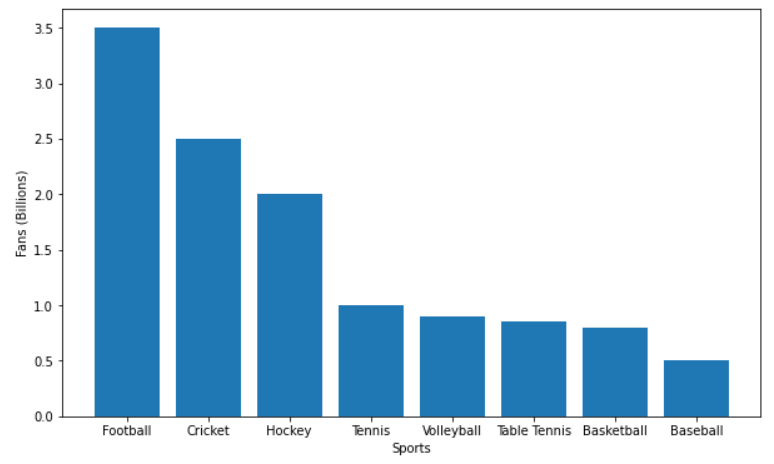
\includegraphics[width=0.8\textwidth]{figures/sports.png}
    \caption{Most popular sports according to number of fans in billions. Source:~\cite{sports}}
    \label{fig:sports}
\end{figure}

Nowadays, there are many different football leagues and events all around the world. The most prestigious leagues are the European ones, such as the English Premier League, German Bundesliga, or Spanish La Liga Primera División. There is also the UEFA Champions League, in which the best teams from all of Europe participate. The World Cup, which is played every four years, is the most famous football event worldwide~\cite{leagues}.

\section{Football Prediction}
The ability to predict the outcome of football games (and other sports events) has become increasingly important in recent times due to the rising number of sports enthusiasts. One significant application of result prediction is (1) the use of bookmakers in correctly setting sport betting odds. With the growing popularity of online betting, more individuals are venturing into this industry, leading to higher stakes, and making it imperative to set the odds correctly. Additionally, with easy access to information and statistics, wrongly set odds can be easily abused. Furthermore, predicting the outcome of a match can (2) aid trainers, managers, and players in adjusting their tactics before the game begins. For example, they can adopt a more defensive approach if the prediction indicates that the opponents have a higher chance of winning. Although predictions should not entirely define their tactics, they can help guide decision-making~\cite{football_prediction}.

The vast majority of models predicting sport results are based on machine learning. Machine learning is a sub-field of artificial intelligence that is able to process the available data and builds a model that approximates or predicts outcomes from yet unseen data. Machine learning can be divided into three main parts: supervised learning, unsupervised learning, and reinforcement learning. Supervised learning is a type of machine learning where an algorithm learns to make predictions by being trained on labeled input/output data. In supervised learning for predicting football match outcomes, the historical match data would be the input, and the labels would be the actual match outcomes (i.e., which team won, lost, or if it was a draw). The algorithm uses this data to identify patterns and relationships between the input and the labels, allowing it to make predictions about the outcomes of future matches based on new input data. 

Sport outcome predictions are most of the time defined as classification problems. In football, one of the three possible outcomes (win, loss, or draw) is typically predicted, and these outcomes are mutually exclusive. This task is obviously harder than predicting one of two classes (win or loss, such as in basketball or volleyball setups). Note that draws also don't happen as often as other outcomes. Thus, the dataset is slightly unbalanced, which makes the task even harder. 

However, sport outcome predictions are sometimes defined as a regression problem, where a numerical value is predicted. In this case, for instance, the numerical value can (a) represent the score of the team, or (b) correspond to the difference between the scores of the two playing teams. When treated as a regression problem, there are two options. The number of goals can be predicted for each team, or the difference between scored goals of each team. The outcome of the game can be directly predicted from the numerical value/s in both cases, but higher accuracy is achieved by using the classification approach most of the time~\cite{ml_review}.

Predicting the outcome of a sport event is generally a hard task because the result can be influenced by many unpredictable aspects such as weather, current mood and performance of a player, injuries, etc. In football, just a single detail can change the shape of the whole game. For example, when one player gets a red card, suddenly the whole team is weakened and may have a hard time winning, even though they were a big favorite. Or just one mistake from a defender can result in a goal from a seemingly harmless situation~\cite{football_prediction}. The average number of goals in a match isn't very high in football. Because of that, one goal decides the outcome of the game quite often. According to~\cite{ml_review}, predicting results of sports with lower scores is generally more difficult. Also, eleven players in each team is such a high number of people. Predicting the performance of an individual person is often easier than predicting the performance of a whole team. Furthermore, the relationships between players and teamwork can also affect the overall performance in such cases~\cite{ml_review}.

There are many machine learning models used for predicting the results of sports games, ranging from simple models like Logistic Regression~\cite{BPL_logistic_regression}, k-Nearest Neighbors (kNN)~\cite{basketball_kNN}, or Random Forest~\cite{football_players}, to more complex models like LogitBoost~\cite{Dutch_football}, Bayesian Network~\cite{Football_Bayesian_network}, or XGBoost~\cite{MLB_regression}, and even the most complex models such as Neural Network~\cite{NBA_convolution} or Support Vector Machine (SVM)~\cite{football_players}. All of these models are used for football prediction, and it is hard to say which one performs the best since they analyze different scenarios, but neural networks are often used and achieve good results.

In this context, football provides a vast array of diverse information that can be utilized as features to feed machine learning models. Probably the most straightforward and easiest to retrieve are the outcomes of the already played matches~\cite{NN_more_sports},~\cite{BPL_ANN_logistic_regression}. The percentage of wins, losses, and draws in the current season can be gathered for both teams, and these percentages can be calculated for home and away games separately as well. Results of previous matches are also simply taken into account, and outcomes of previous encounters between the playing teams can also be important~\cite{Dutch_football}. Next are the statistics from the games themselves~\cite{NFL_first_study},~\cite{basketball_kNN}, which can include the number of goals, shots, corners, free kicks, fouls, etc. These statistics can reflect the form of the team if it is not visible in the outcomes, and they can also reflect the playstyle of the teams, which can be meaningful for the outcome.

Moreover, other ad-hoc data is frequently used as features, such as offensive and defensive strength from the FIFA game~\cite{BPL_logistic_regression} or differently calculated coefficients representing the offensive and defensive strength of the teams~\cite{BPL_ANN_logistic_regression}. The number of days the team can rest or the distance between the home and away team's city can also be used~\cite{Dutch_football}, and sometimes even the betting odds can be included~\cite{NBA_convolution}. Although this usually helps with accuracy, such information may not be very useful when the aim is to beat or help the bookmakers.

Thus, feature selection is often used to improve the prediction of football results. This technique is an important part of machine learning because it reduces dimensionality and removes redundant features. Feature selection methods can be divided into three categories: filter methods, which select the features based on dependency on the outcome variable; wrapper methods, where the feature selection is based on the performance of the model; and embedded methods, which select the features during the execution of the modeling algorithm. Specific feature extraction methods used for football prediction include Principal Component Analysis (PCA)~\cite{Dutch_football}, Signal-to-Noise Ratio (SNR)~\cite{snr}, Correlation-based Feature Subset selection (CFS)~\cite{cfs}, or ReliefF~\cite{Dutch_football}.

Note, however, that some of the more complicated models used to predict football outcomes also use statistics of individual players who play in the predicted match~\cite{football_players},~\cite{NBA_convolution}. These statistics can include, for example, the number of goals, number of shots, number of correct passes, number of fouls, etc. These models usually treat those features differently and do some preprocessing of them inside the model.

A summary of a general framework for predicting sport results described in the section above is pictured in Figure~\ref{fig:ml_diagram}.

\begin{figure}[h]
    \centering
    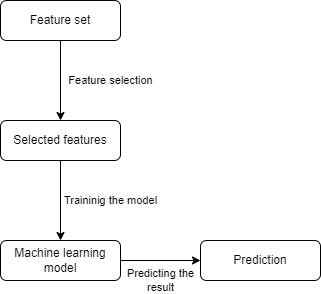
\includegraphics[width=0.5\textwidth]{figures/ml_diagram.png}
    \caption{General machine learning pipeline for sport result prediction. The most relevant features are selected from the candidate feature set. The chosen machine learning model is trained on the training data consisting of the selected features. The trained model can then predict the results of previous matches.}
    \label{fig:ml_diagram}
\end{figure}

\section{Contributions}

The focus of this thesis is to predict the outcomes of football matches based on data from previous matches. Despite the significant progress made by machine learning approaches in football, there are still several unanswered research concerns. To the best of my knowledge, no previous work has explored the use of tensor completion to enhance football prediction. By treating each season as a slice of a 3D tensor, tensor completion can help identify patterns between seasons that may be useful in forecasting results for the current season. For example, a team's past performance could be an indicator of their potential performance in the present season. Additionally, tensor completion can aid in accounting for changes in team quality over time. Moreover, it can find patterns in the previous encounters of certain teams.

This work concerns the validation of the following thesis:

\vspace{0.5cm}
\hfill\begin{minipage}{0.90\textwidth}
``The three-dimensional tensor completion problem, where each slice represents a win-lose-draw matrix for a given season with home and away teams as entities in the rows and columns, is an accurate model for predicting football outcomes. It achieves state-of-the-art performance compared to existing methods in the literature when exposed to comparable data scenarios while still maintaining interpretability. Furthermore, incorporating embeddings extracted from tensors that model football predictions improves the accuracy of relevant methods for football prediction.''
\end{minipage}
\vspace{0.5cm}




{
\definecolor{shadecolor}{rgb}{0.8,0.8,0.8}
\begin{shaded*}

\noindent \textbf{Scientific Contributions}

\noindent This thesis regards the following scientific contributions:

%\singlespacing
\begin{enumerate}[\hspace{20pt}(1)]
    \item A comprehensive literature review of football result prediction and sports outcome prediction in general, summarizing the main methods used in related scenarios (see Sections~\ref{applications} and~\ref{summary}). Additionally, a review and description of various algorithms for tensor completion, which were later utilized for prediction purposes (see Section~\ref{tensor_algs}).

    \item A detailed account of the machine learning approaches implemented for the proposed methods and baselines (see Section~\ref{methods}), providing a deeper insight into the models used and their potential implications for the prediction tasks at hand.
    
    \item Sourcing and preparation of data for four European leagues, as well as the Brazilian league, from various sources, followed by statistical analysis of the retrieved dataset (see Sections~\ref{dataset} and~\ref{dataset_analysis}).

    \item Introduction and implementation of a novel approach for predicting the results of football games based on tensor completion (see Section~\ref{model}), as well as implementation of baseline methods as outlined in relevant papers, ensuring that they utilized similar features, comparable amounts of data, and the same architecture for the model (see Section~\ref{baselines}).

    \item Extraction of embeddings that represent the performance of teams in both their home and away games using tensor completion and the singular value decomposition (SVD) of the last slice (the predicted season) (see Section~\ref{embeddings}). These vectors were then employed to build models that incorporate the tensor completion embeddings (see Section~\ref{vectors}). The usefulness of these embeddings was further demonstrated, along with their interpretability properties (see Section \ref{clustering}).
\end{enumerate}


\end{shaded*}

}

%---------------------------------------------------------------
\chapter{Theoretical Background}
\label{ter_back}
%---------------------------------------------------------------
\section{Applications}
\label{applications}
In this section, I will introduce some of the most important works dealing with predicting sport outcomes. Many papers on football prediction and predicting sport results in general, have been written over the years. The first paper covering this topic was published at the end of the twentieth century~\cite{NFL_first_study}. Since then, a lot of different machine learning models and techniques have been used for predicting sport results. Data scientists are coming up with more and more complex approaches. However, it is challenging to compare the results of these works for accuracy because different testing datasets are used in every paper.

\subsection{Football Prediction}
In the field of predicting the outcomes of football matches, various works can be found. In 2013, F. Owramipur et al. predicted the results of the Spanish La Liga Primera División with a Bayesian Network in~\cite{Football_Bayesian_network}. They found the main factors that affect football results and divided them into non-psychological and psychological factors. However, the model could only predict the results of a single team, so only Barcelona games were predicted. Although the authors achieved an impressive accuracy of 92\%, the results were limited since they only predicted matches of one team.

C. P. Igiri and E. O. Nwachukwu predicted the outcomes of matches in the English Premier League in 2014 in~\cite{BPL_ANN_logistic_regression}. For this, they applied two machine learning models: Logistic Regression and Neural Network. Nine different features, such as scored goals, achieved corners, or attack strength, were used for the prediction. The dataset was extracted only from the 2014-15 season. Regarding the models' results, the Neural Network had an accuracy of 85\%, and Logistic Regression achieved an accuracy of 93\%. Logistic Regression can only predict win or loss, while the Neural Network can predict all possible outcomes: win, loss, or draw.

In~\cite{Dutch_football} from 2015, N. Tax and Y. Joustra used several models including Naive Bayes, LogitBoost, Neural Network, Random Forest, and Decision Tree for predicting Dutch Eredivise match outcomes. They applied three dimensionality reduction techniques, namely Principle Component Analysis, Sequential Forward Selection, and ReliefF. The authors compared the models using only public statistics, only betting odds, and both. They took into account 13 seasons (2000-2013). The best accuracy in statistics data models was achieved by Naive Bayes with PCA and Neural Network, which both reached 54.7\%. The betting odds model achieved slightly higher accuracy, and the hybrid model achieved the highest accuracy, but the differences were very small.

In 2016, D. Prasetio and M. Harlil used Logistic Regression for predicting the outcomes of Premier League games in~\cite{BPL_logistic_regression}. They used only four features gathered from the video game FIFA for predicting. The authors utilized five seasons of data (2010-11 up to 2014-15). The best achieved accuracy was 69.5\%. The model could only predict win or loss, as in the previous paper using Logistic Regression.

J. Stübinger, B. Mangold, and J. Knoll in~\cite{football_players} predicted the results of European first and second leagues from five countries. They employed Random Forest, Boosting, SVM, and Linear Regression and used a large number of features. The authors incorporated game characteristics and proportions of all players from both teams. They gathered data from games from 2006 to 2018. The ensemble of all models achieved the best results with an accuracy of 81.77\%. The authors conducted a financial analysis, and the ensemble strategy achieved statistically and economically significant returns of 1.58\% per match.

\subsection{Other Sports Prediction}
The field of other sports results prediction using machine learning has seen many published works. The first study in this field was conducted by M. C. Purucker in 1996~\cite{NFL_first_study}. They predicted outcomes of American football NFL with a Neural Network, using only four, and later five, features. Both supervised and unsupervised learning were applied, with the former yielding better results. Only data from the 1994 season was used, and the best accuracy achieved was 78.6\%, but it was based on only fourteen samples.

In 2008, A. McCabe and J. Trevathan~\cite{NN_more_sports} predicted the results of four sports (rugby, Australian football, super rugby, and football) with one model. They also chose a Neural Network and used ten features, which were the same for each sport. They employed a three-layer Multi Layer Perceptron (MLP) with nineteen, ten, and one neuron. The authors collected data from at least three seasons for each sport, with the most seasons (six) used for rugby. The best achieved accuracy was 75.4\% in super rugby, and the results were comparable to human tippers.

In 2018, T. Tran predicted NBA matches using matrix factorization in~\cite{NBA_matrix_factorization}. The entry (i, j) in the matrix corresponds to team i's score when playing against team j. The matrix was factorized into latent matrices U and V, representing offense and defense latent vectors, respectively. Probabilistic matrix factorization (PMF) was used to incorporate the fact that scores will differ each time two teams play each other. Supplementary information, such as the date of the game and information about home/away teams, was also incorporated into the PMF model. The author experimented with different numbers of seasons, but the best results were achieved with just the last season (2014-15), with a best accuracy of 72.1\%.

In 2018, T. Elfrink predicted baseball outcomes, specifically the MLB, in~\cite{MLB_regression}. They used GLM, XGBoost, Random Forest, and Boosted Logistic Regression. The author gathered 164 different features and treated the problem as classification and as regression. Data from games played between 1930 and 2016 were used. The best accuracy was 55.52\% achieved by XGBoost. This result is not good enough to beat betting companies.

T. Horvat, J. Job, and V. Medved predicted the results of Basketball Euroleague with kNN in~\cite{basketball_kNN}. The authors used nine basic basketball statistics and proposed two variants of data preparation. The first variant groups the statistics into offense and defense groups, and the second one divides them into six groups. Feature selection was experimented with, but it did not increase the accuracy. The statistics from seasons 2012-2013 to 2016-2017 were used. The highest accuracy was 83.39\%, achieved by dividing the statistics into offense and defense groups.

In \cite{NBA_convolution}, O. Hubáček, G. Šourek, and F. Železný predicted the outcomes of NBA with a Neural Network. The authors used statistics about teams and players for prediction and applied a convolutional layer for player-data processing in combination with classic dense layers. The data processing from players is shown in figure \ref{fig:conv}. The authors focused on decorrelating the model with bookmakers' predictions. The best accuracy was 68.7\%. Although the accuracy is slightly lower than that of the bookmakers' model, it was shown that decorrelation helps to make a bigger profit. 

\begin{figure}[h]
    \centering
    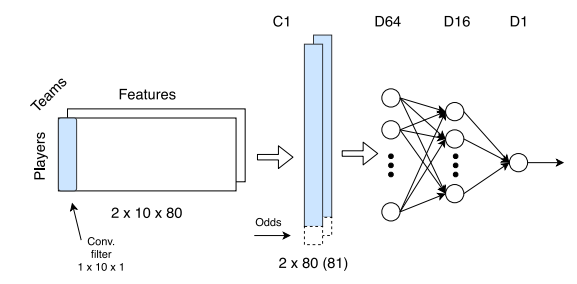
\includegraphics[width=0.8\textwidth]{figures/conv.png}
    \caption{Player data processing from \cite{NBA_convolution}}
    \label{fig:conv}
\end{figure}

\section{Methods}
\label{methods}
Many different machine learning algorithms and techniques have been applied for sports results prediction. Based on my literature search, the most frequently used models are Neural Network and Logistic Regression, respectively. Other models used were, for example, Naive Bayes, Random Forest, or matrix factorization. In some works, the authors applied a batch of algorithms on their experimental evaluation and then output the best model. Here, we will briefly present the theoretical backgrounds of the methods related to this thesis.

\subsection{Logistic Regression}
\textbf{Basic background:} Logistic Regression is a model for binary classification: $$P(Y = 1|\boldsymbol{x},\boldsymbol{w}) = \frac{\e^{\boldsymbol{w}^T\boldsymbol{x}}}{1 + \e^{\boldsymbol{w}^T\boldsymbol{x}}},$$ where $Y$ is the predicted variable with possible values of 0 and 1, $\boldsymbol{x}$ is the vector of features, and $\boldsymbol{w}$ is the vector of weights. Both vectors are of length $p + 1$, where $p$ is the number of features, and $x_0 = 1$. 

During training, the weights $\boldsymbol{w}$ are optimized. This is done with Maximum Likelihood Estimate (MLE). Let $$p_{Y_i}(\boldsymbol{x}_i, \boldsymbol{w}) = P(Y = Y_i|\boldsymbol{x}_i, \boldsymbol{w})$$ be the probability of the data point $\boldsymbol{x}_i$ with a value of the predicted variable of $Y_i$ for a given $\boldsymbol{w}$. The probability of all data points combined should be the highest possible, so the following function is being maximized: $$L(\boldsymbol{w}) = \prod_{i = 1}^N p_{Y_i}(\boldsymbol{x}_i, \boldsymbol{w})$$ and after applying logarithm: $$l(\boldsymbol{w}) = \sum_{i = 1}^N Y_i \boldsymbol{w}^T\boldsymbol{x} - \ln{(1 + {\e}^{\boldsymbol{w}^T\boldsymbol{x}})},$$ where $N$ is the number of samples. The gradient of this function can be written as: $$\nabla l(\boldsymbol{w}) = \boldsymbol{X}^T(\boldsymbol{Y} - \boldsymbol{P}),$$ where $\boldsymbol{P} = (p_1(\boldsymbol{x}_1, \boldsymbol{w}), p_1(\boldsymbol{x}_2, \boldsymbol{w}), \dots, p_1(\boldsymbol{x}_N, \boldsymbol{w}))^T$. The maximum should be found with a solution to the equation $\nabla l(\boldsymbol{w}) = 0$, but this equation can't be explicitly solved. The maximum has to be approximated with numerical approximate methods, such as gradient rise or Newton's method~\cite{lr}.

\noindent \textbf{Related works:} C. P. Igiri and E. O. Nwachukwu in~\cite{BPL_ANN_logistic_regression} and D. Prasetio and M. Harlil in~\cite{BPL_logistic_regression} used Logistic Regression to predict sport results. In both papers, the outcomes of English Premier League matches were predicted. The authors did not specify how they dealt with draws in either of the papers, but since logistic regression is a model for binary classification, a reasonable assumption is that they ignored all matches that ended in a draw.

In~\cite{BPL_ANN_logistic_regression}, the authors used the following features: goals, shots, corners, odds, attack strength, players’ performance index, managers’ performance index, managers’ win, and streak - all for the home and away team. The dataset consisted of 110 matches played in the 2014/15 Premier League season. They gathered the data from different sources and processed it with Knowledge Discovery in Database technique. The data was cleaned and consolidated. For imputing the missing values, they used Neural Network. They also did weighting optimization with Genetic Algorithm (GA) and parameter optimization with an evolutionary approach, which was used to adjust the learning rate, momentum, and other parameters. With Logistic Regression, they achieved an accuracy of 93\%, which was higher than with the Neural Network, which they also used.

In~\cite{BPL_logistic_regression}, the authors gathered data from the FIFA game. They used only home offense, home defense, away offense, and away defense as features. The testing dataset consisted of matches from the 2015/16 season. They experimented with the amount of data to train the model on. The best results were achieved with training data from the 2010/11 to 2014/15 seasons. When they added the testing season to the training dataset, the accuracy decreased, which could be a sign that the model is not prone to overfitting. The achieved accuracy was 69.5\%. The biggest coefficients in the Logistic Regression model were for the home defense and away defense features. They stated that these features are the most important ones.

\subsection{Neural Network}
\textbf{Basic background:} Neural Network is a complex machine learning algorithm. The basic part of a Neural Network is a single neuron. In the neuron, all the inputs are multiplied by weights, summed up, a bias is added, and an activation function is applied to the result. The output of the neuron is then defined as: $$f(\boldsymbol{w}^T \boldsymbol{x} + w_0),$$ where $f$ is the activation function, $\boldsymbol{w}$ and $\boldsymbol{x}$ are the same as in the Logistic Regression vector of weights and vector of features (inputs), and $w_0$ is the bias. The expression $f(\boldsymbol{w}^T \boldsymbol{x} + w_0)$ is often signified as $\xi$ and is called the inner potential of the neuron. The single neuron can only solve linear functions. That's why neurons are connected in layers. A Multi-Layer Perceptron (MLP) consists of layers of neurons. The outputs of neurons in one layer are the inputs of neurons in the next layer. All the layers except the input layer and the output layer are called hidden layers. In Figure~\ref{fig:mlp}, an MLP with one hidden layer can be seen. 

\begin{figure}[h]
    \centering
    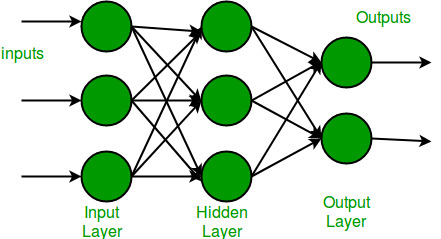
\includegraphics[width=0.8\textwidth]{figures/mlp.jpg}
    \caption{Multi-Layer Perceptron. Source: \cite{nn_pic}}
    \label{fig:mlp}
\end{figure}

It has been proven that an MLP with just one hidden layer can approximate any continuous function with arbitrary accuracy. In the real world, networks with more hidden layers are created, however. Deep learning works with Neural Networks with more than three hidden layers. The problem with these complex Neural Networks was the training, which took a long time. Backpropagation, which is used for training Neural Networks, wasn't discovered until the 80s. For backpropagation to work, the Neural Network as a function of the parameters has to be fully differentiable. For this purpose, suitable activation functions have to be used. Many different activation functions are being experimented with. The most common ones include hyperbolic tangents: $$f(\xi) = \frac{\e^\xi - \e^{-\xi}}{\e^\xi + \e^{-\xi}}$$ or Rectified Linear Unit (ReLU):
\[   
f(\xi) = 
     \begin{cases}
       \xi &\quad\text{if } \xi\ge 0\\
       0 &\quad\text{otherwise.}\\
     \end{cases}
\]
This function is not differentiable at zero, but it has a non-zero derivative in the positive domain, which is the important part. In the output layer, different activation functions are applied to convert the calculated values to values from which the prediction can be made. Mostly one of three activation functions is applied in the output layer. The identity function ($f(\xi) = \xi$) is used for regression tasks. There is basically one neuron with no activation function. For binary classification, sigmoid is used: $$f(\xi) = \frac{\e^\xi}{1 + \e^\xi}.$$ There is one neuron with this activation function, and its value represents the probability of class 1, the same as in logistic regression. For classification into more classes, there is the softmax function. In the output layer, there are the same number of neurons as the number of classes. Each neuron has the softmax activation function: $$f_i(\boldsymbol{\xi}) = \frac{\e^\xi_i}{\e^{\xi_1} + \e^{\xi_2} + \dots + \e^{\xi_c}},$$ where $\boldsymbol{\xi}$ is the vector of the inner potentials of the output neurons and $c$ is the number of classes. The output of the $i$-th neuron $f_i(\boldsymbol{\xi})$ is interpreted as the probability of the $i$-th class.

While training, the loss function is being minimized, which measures how well the Neural Network works. For regression problems, the square error is calculated: $$L(Y, \hat{Y}) = (Y - \hat{Y})^2,$$ where $Y$ is the true value, and $\hat{Y}$ is the prediction. For binary classification, binary cross-entropy is used: $$L(Y, \hat{p}) = -Y\log{\hat{p}} - (1 - Y)\log{(1 - \hat{p})},$$ where $\hat{p} = \hat{P}(Y = 1|\boldsymbol{X} = \boldsymbol{x})$. With classification into $c$ classes, categorical cross-entropy is measured: $$L(Y, \hat{\boldsymbol{p}}) = -\sum_{j = 1}^c m_j \log{\hat{p}_j} = -\log{\hat{p}_Y},$$ where $\hat{p}_j = \hat{P}(Y = j|\boldsymbol{X} = \boldsymbol{x})$, $\boldsymbol{\hat{p}_j} = (\hat{p}_1, \hat{p}_2, \dots, \hat{p}_c)$, and $m_j = 1$ if $Y = j$ and $m_j = 0$ otherwise.

Let $g(\boldsymbol{x};\boldsymbol{w})$ be the Neural Network written as a function with parameters $\boldsymbol{w}$ and inputs $\boldsymbol{x}$. During training, the average of the loss function on the training set is minimized: $$J(\boldsymbol{w}) = \frac{1}{N}\sum_{i = 1}^N L(Y_i, g(\boldsymbol{x_i};\boldsymbol{w}))$$ with respect to the parameters $\boldsymbol{w}$. The minimization is done by gradient descent. Calculating the gradient takes advantage of the rule for calculating the derivative of nested functions. The gradient is calculated gradually from the output layer to the input layer by multiplying and summing the partial derivatives~\cite{nn}.

\noindent \textbf{Related works:} M. C. Purucker in~\cite{NFL_first_study}, A. McCabe and J. Trevathan in~\cite{NN_more_sports}, C. P. Igiri and E. O. Nwachukwu in \cite{BPL_ANN_logistic_regression}, and O. Hubáček, G. Šourek, and F. Železný in \cite{NBA_convolution} used Neural Networks for sport match outcome prediction.

In~\cite{NFL_first_study}, the authors predicted American football matches of the NFL. They experimented with several types of Neural Networks, including Hamming, Adaptive Resonance Theory (ART), Kohonen Self-Organizing Map (SOM), and Back-Propagation (BP). They also used supervised and unsupervised learning. They gathered the following five features: yards gained - yards allowed, rushing yards gained - allowed, turnover margin, and possession time margin in minutes. The best results were achieved with a BP Neural Network using supervised learning. The authors experimented with several architectures of the BP Neural Network, but the predictions were very similar, so they chose a simple architecture with five inputs, one output, and no hidden neurons. They retrieved the data from the 1994 NFL season and used week sixteen as the testing set, where the BP Neural Network predicted eleven out of fourteen games correctly, giving an accuracy of 78.6\%.

In~\cite{NN_more_sports}, A. McCabe and J. Trevathan predicted outcomes of games in four different sports with one Neural Network. The sports and leagues were rugby - National Rugby League (NRL), Australian football - Australian Football League (AFL), super rugby - Super 12 and Super 14, and football - English Premier League (EPL). They extracted features from various data sources, including Points-for, Points-against, Overall Performance, Home Performance and Away Performance, Performance in Previous Game, Performance in Previous n Games, Team Ranking, Points-for in Previous n Games, Points-against in Previous n Games, and Location. They used MLP and experimented with Back Propagation and Conjugate Gradient Method, and the first optimization method resulted in slightly better metrics. The MLP had three layers with nineteen neurons in the input layer, ten in the hidden layer, and one in the output layer. The Neural Network returned a number between 0 and 1 for each team, and the team with a higher number was predicted as the winner. For each league, at least three seasons were used as the dataset. For NRL, six seasons were taken into account, which was the highest from all sports. The model achieved an accuracy of 68.1\% for AFL, 67.2\% in NRL, 75.4\% in super rugby, and 58.9\% in EPL.

In~\cite{NBA_convolution}, the authors applied a Neural Network to predict NBA matches. The data was gathered from seasons 2000 to 2014, with each season providing around a thousand games. They used a large number of features to measure the team's performance in the current season for both the home and away teams. They also incorporated features representing the performance of individual players. The model consisted of a convolutional layer followed by three dense layers. The purpose of the convolutional layer was to deal with the large number of player-based features. It served as a bridge from player-level variables to a team-level representation. They designed a strategy for bet distribution according to the bookmakers' odds and the model's prediction. The best achieved accuracy without using the odds as features was 68.7\%. Although this is slightly lower than the accuracy of the bookmakers' model and the model that uses the odds, it is less correlated with the bookmakers' model and thus makes a bigger profit.

In~\cite{BPL_ANN_logistic_regression}, a Neural Network was used in addition to the Logistic Regression model discussed earlier. The Neural Network achieved an accuracy of 85\%, which was lower than that of the Logistic Regression model. However, the Neural Network can predict draws, which the Logistic Regression model cannot.

\subsection{Matrix Factorization}
\label{matrix_fac}
 \textbf{Basic background:} Matrix factorization is a method that expresses a given matrix $\boldsymbol{R}$ as a product of two lower dimensional matrices. The idea is to find lower dimensional matrices $\boldsymbol{U} \in \mathbb{R}^{m \times d}$ and $\boldsymbol{V} \in \mathbb{R}^{d \times n}$ for a given matrix $\boldsymbol{R} \in \mathbb{R}^{m \times n}$ so that the elements of $\boldsymbol{R}$ are well approximated by the matrix $\boldsymbol{U} \boldsymbol{V}$. This idea is illustrated in Figure~\ref{fig:mf}.
\begin{figure}[h]
    \centering
    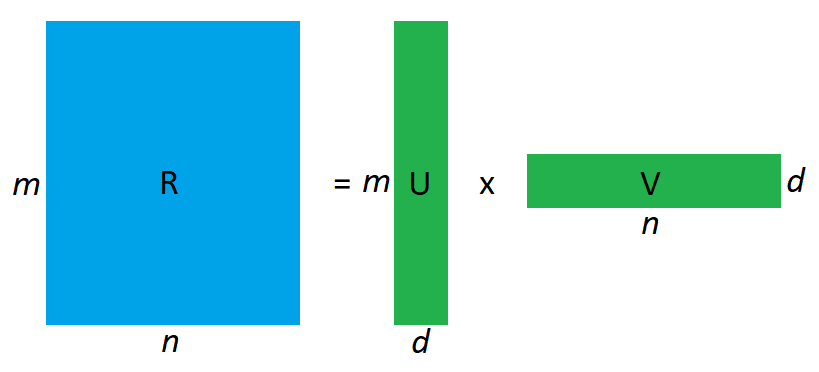
\includegraphics[width=0.6\textwidth]{figures/mf_my.PNG}
    \caption{Matrix $\boldsymbol{R}$ is approximated by matrix $\boldsymbol{U} \boldsymbol{V}$.}
    \label{fig:mf}
\end{figure}
If there are missing values in matrix $\boldsymbol{R}$, the approximation $\boldsymbol{U} \boldsymbol{V}$ can be used to fill (predict) those values. The matrices $\boldsymbol{U}$ and $\boldsymbol{V}$ are then chosen to approximate only the known entries of $\boldsymbol{R}$. This is called matrix completion.

Let $p_u$ be the $u$-th row of matrix $\boldsymbol{U}$, $q_i$ the $i$-th column of matrix $\boldsymbol{V}$, and $K$ a set of pairs $(u, i)$ such that $r_{u, i}$ is known, where $r_{u, i}$ is the element of matrix $\boldsymbol{R}$ in the $u$-th row and $i$-th column. The approximation of $r_{u, i}$ is then given by the number $p_u^T q_i$. The error of approximation is measured by the squared residual: $$(r_{u, i} - p_u^T q_i)^2.$$ The matrices $\boldsymbol{U}$ and $\boldsymbol{V}$ are found by solving the optimization task: $$\arg \min_{\boldsymbol{U}, \boldsymbol{V}} \sum_{(u, i) \in K} (r_{u, i} - p_u^T q_i)^2.$$ To solve this task, gradient descent or alternating least squares method can be used. With gradient descent, the matrices are randomly set and then updated step by step according to the gradient. With alternating least squares method, one of the matrices is always fixed and the other is optimized. The matrices are found for a given $d$, which is a hyperparameter. Since the ground-truth assumption is that $\boldsymbol{R}$ is of low-rank, $d$ must be a positive integer significantly smaller than $m$ and $n$.

Matrix factorization is often applied in recommender systems. In this case, $\boldsymbol{R}$ is a rating matrix where $r_{u, i}$ represents the rating of user $u$ on item $i$. There is usually a huge number of users and items, but every user rates only a few items. Because of that, the rating matrix is very sparse. The goal of matrix factorization here is to predict the missing ratings~\cite{mf}.

\noindent \textbf{Related works:} T. Tran in~\cite{NBA_matrix_factorization} used matrix factorization to predict NBA outcomes. They put the results of the matches into a matrix, so each entry $(i, j)$ in the matrix represents team $i$’s score when playing against team $j$, and vice versa for entry $(j, i)$. They assumed that each team can be described with two vectors representing its offense and defense. To learn these vectors, they applied matrix factorization to find matrices $\boldsymbol{U}$ and $\boldsymbol{V}$, such that the matrix $\boldsymbol{U} \boldsymbol{V}$ approximates the original matrix. Their model uses gradient descent for optimization. Teams play against each other multiple times, so they initially kept the average scores of the mutual matches in the matrix.

Moreover, they used PMF to address this issue, which slightly increased accuracy. They also applied Dependent Probabilistic Matrix Factorization (DPMF) to incorporate supplementary information into the model. They included information about which team plays as the home team and the date and time of the game. The author experimented with the amount of training data. They had data from seasons 1985/86 to 2015/16 available and used the last season for evaluation. The highest accuracy was achieved when considering the 2014/15 season as training data only. They also experimented with the value $d$, which is the dimension of the matrices $\boldsymbol{U}$ and $\boldsymbol{V}$. The best results for DPMF were achieved for $d=5$. The best accuracy was reached with DPMF of 72.1\%.

\subsection{PCA with Naive Bayes}
In~\cite{Dutch_football}, the authors applied several models for predicting football outcomes and found that Naive Bayes with PCA achieved state-of-the-art accuracy. Based on this, I have included this model as one of the baselines in my thesis.

\noindent \textbf{Basic background:} Naive Bayes is a basic probabilistic model for classification that uses Bayes' theorem: $$P(Y = y | \boldsymbol{X} = \boldsymbol{x}) = \frac{P(\boldsymbol{X} = \boldsymbol{x} | Y = y)P(Y = y)}{P(\boldsymbol{X} = \boldsymbol{x})}.$$ The goal is to find $y$ for which this probability is the highest. The expression $P(\boldsymbol{X} = \boldsymbol{x})$ is the same for every $y$, so it is ignored. Naive Bayes assumes that all features are conditionally independent given $Y=y$. This assumption is often incorrect, but Naive Bayes often gives good results. The prediction is determined as follows: $$\hat{Y} = \arg \max_{y \in Y} \prod_{i = 1}^p P(X_i = x_i | Y = y)P(Y = y).$$ The features in Naive Bayes are treated as completely independent. This helps mitigate problems with dimensionality, and the amount of data needed for reasonable predictions does not scale with increasing dimension.

Different probability distributions are used for estimating $P(X = x | Y = y)$ depending on the type of feature $X$. For binary features, Bernoulli distribution with parameter $p_y$ is applied, where $p_y = P(X = 1 | Y = y)$. For categorical features with values $c_1, c_2, \dots, c_k$, multinomial distribution with parameter $\boldsymbol{p_y}$ is used, where $\boldsymbol{p_y} = (p_{1, y}, p_{2, y}, \dots, p_{k, y})^T$ and $p_{j, y} = P(X = c | Y = y)$.

For continuous features, the probability $P(X = x | Y = y) = 0$ for every $x$ and is unusable. Instead, the probability density $f_{X|y}(x)$ is taken into account. The prediction is then defined as: $$\hat{Y} = \arg \max_{y \in Y} \prod_{i = 1}^l P(X_i = x_i | Y = y) \prod_{i = l + 1}^p f_{X_i|y_i}(x)P(Y = y),$$ where $X_1, X_2, \dots, X_l$ are discrete features and $X_{l + 1}, X_{l + 2}, \dots, X_p$ are continuous features. A Gaussian distribution $\mathcal{N}(\mu_y, \sigma_y^{2})$ with a mean value of parameter $\mu_y$ and a variance of parameter $\sigma^2_y$ is often used to approximate the distribution $X | Y = y$. The probability density is then defined as: $$f_{X|y}(x) = \frac{1}{{\sigma_y \sqrt {2\pi } }}e^{{{ - \left( {x - \mu_y } \right)^2 } \mathord{\left/ {\vphantom {{ - \left( {x - \mu_y } \right)^2 } {2\sigma_y^2 }}} \right. \kern-\nulldelimiterspace} {2\sigma_y^2 }}} \cite{nb}.$$

PCA is one of the most common dimensionality reduction techniques. Let $V$ be a $q$-dimensional vector subspace of the vector space $\mathbb{R}^p$. Every point $x \in \mathbb{R}^p$ can be decomposed into: $$x = v_x + u_x,$$ where $v_x$ is a point of $V$, and $u_x$ is perpendicular to $V$. The point $v_x$ is called the orthogonal projection of the point $x$ onto the subspace $V$. Let $b_1, b_2, \dots, b_p$ be an orthonormal basis of $\mathbb{R}^p$, where $b_1, b_2, \dots, b_q$ forms a basis of $V$, and $b_{q+1}, b_{q+2}, \dots, b_p$ are perpendicular to $V$. Every point $x \in \mathbb{R}^p$ can be expressed as: $$x = v_x + u_x = \tau_1 b_1 + \tau_2 b_2 + \dots + \tau_q b_q + \tau_{q+1} b_{q+1} + \tau_{q+2} b_{q+2} + \dots + \tau_p b_p,$$ where $\tau_i = x^T b_i$. The projection $v_x$ of point $x$ onto subspace $V$ can be described by vector $t_x = (\tau_1, \tau_2, \dots, \tau_q)^T \in \mathbb{R}^q$. This vector can be written as a matrix product: $$t_x = \boldsymbol{V}^T x,$$ where $\boldsymbol{V} \in \mathbb{R}^{p \times q}$ is a matrix with vectors $b_1, b_2, \dots, b_q$ as columns. For a dataset represented as a matrix $\boldsymbol{X}^{N \times p}$ with $N$ data points and $p$ features, the transformed dataset is defined as: $$\boldsymbol{T}_q = \boldsymbol{X} \boldsymbol{V}.$$

PCA finds the projection for each $q$, which minimizes the square error of the projection of dataset $\boldsymbol{X}$ onto the $q$-dimensional subspace $V$. Firstly, each point of the dataset is centered as: $$x'_i = x_i - \bar{x},$$ where $\bar{x}$ is the sample mean of the dataset. For the orthogonal decomposition of point $x'_i = v_{x'_i} + u_{x'_i}$, the following expression is minimized: $$\sum_{i=1}^N ||x'_i - v_{x'_i}||^2 = \sum_{i=1}^N ||u_{x'_i}||^2.$$ The solution uses the eigenvectors $b_1, b_2, \dots, b_p$ of the matrix $\frac{1}{N-1}X'^T X'$ as the orthonormal basis. Subspace $V$ and matrix $\boldsymbol{V}$ are then formed by the first $q$ vectors of this basis~\cite{pca}.

 \noindent \textbf{Related works:} N. Tax and, Y. Joustra in~\cite{Dutch_football}, T. Elfrink in~\cite{MLB_regression} and J. Stübinger, B. Mangold and J. Knoll in~\cite{football_players} used many machine learning models for sport prediction.
 
 In~\cite{Dutch_football} from 2015 the authors predicted the outcomes of Dutch Eredivisie football league matches. They experimented with many combinations of machine learning algorithms and dimensionality reduction techniques. For the machine learning algorithms, they used, for example, Random Forest, LogitBoost, DTNB, MLP, Naive Bayes, FURIA or Decesion Tree. As dimensionality reduction techinques, they have chosen Principle Component Analysis, Sequential Forward Selection and ReliefF.
 
 The authors have created several feature sets. The public feature set contains public data without the bookmakers odds. Betting odds feature set consists only of the odds and hybrid feature set contains both. For the public features they gathered many statistics from previous results, from the games themself and others such as average number of goals, average goals by top-scorer, average assists by top-assist, results of previous matches, percentage of wins this season, percentage of wins in earlier encounters, number of days since previous match, number of days coached by current coach, distance between home and away city and many more. For the betting odds features they used the odds from Gamebookers, Bet\&Win and Betbrain for the result of the match and for the Asian handicap.
 
 The authors gathered data from seasons 2000/01 to 2012/13. First seven seasons were used for training and the rest for evaluation. For the public model the highest achieved accuracy was 54.7\% by MLP with PCA with three and seven components by Naive Bayes with PCA with three components. Highest accuracy for the betting odds model was achieved by FURIA - 55.3\%. For the hybrid model LogitBoost with ReliefF with five attributes had the highest accuracy of 56.05\%. McNemar’s test hasn't showed significant difference between the models, but it can be seen, that adding public data to the betting odds model can increase the accuracy.

\subsection{Further Methods}
As stated before, some works have used a set of machine learning models for sports prediction. Unlike my work, which aims to understand the phenomenon of predicting football outcomes using a single model (tensor completion), other studies focus on analyzing football predictions using various methods. To accomplish this, these studies typically prepare a dataset and then run multiple models, comparing and contrasting the results. In the following section, we will provide a brief overview of some of these works.

\noindent \textbf{Related works:} In~\cite{MLB_regression}, the author predicts baseball games from the MLB. They experimented with four machine learning models: Generalized Linear Model, Random Forest, XGBoost, and a Boosted Logistic Regression. They gathered data from years 1930 to 2016. The last season is used as the validation dataset. The data was stored in the form of events. One event represents one at-bat in a game. Each event has over 164 different features, and each year has around 200,000 different events. They extracted statistics of the teams' performance from these events. The author also applied Independent Component Analysis, which added new features that are linear combinations of the original ones. They treated the task as a binary classification problem and also as a regression problem, where they predicted the difference between scores. The best-achieved accuracy was 55.52\% by the XGBoost model, treating the task as a binary classification problem.

In~\cite{football_players} from 2019, the authors predicted the results of ten European football leagues. It was the first and second leagues from England, Germany, Spain, Italy, and France. They gathered the data from seasons 2006/07 to 2017/18. The whole dataset consists of 47,856 matches. They used Random Forest, Boosting, Support Vector Machines, and Linear Regression. They also created an ensemble of those four models. As features, they used statistics of each individual player. They got the data from the FIFA game, where they gathered statistics of 19,998 different players. There were, for example, stats like body measures, pass accuracies, agility, reaction, or aggression. They made a betting strategy according to the machine learning models' predictions. They compared this strategy to some baselines, such as always bet on the home team. The authors achieved an accuracy of 81.77\% with the ensemble of all models. The betting strategy based on this model made a profit of 1.58\% per match.

\section{Literature Summary}
\label{summary}

Table~\ref{table:works} summarizes the main related works in the field of predicting football outcomes. Our study investigates the phenomenon of football prediction using a novel approach based on tensor completion, which, to the best of our knowledge, has not been implemented before in this context. Our work differs from the most comparable approach in the literature \cite{NBA_matrix_factorization}, which is based on matrix factorization. A notable advantage of our model is that it considers all previous seasons concurrently, whereas the previous work only considers one season at a time. This innovative feature makes our work a distinctive contribution to the field of sports result prediction.

In this thesis, we evaluate the tensor completion model in two scenarios, considering four leagues, 25 seasons, and predicting wins, losses, and draws. First, we (1) compare it to state-of-the-art methods that use similar information as a setup for direct outcome prediction. Second, we (2) analyze the impact of using tensor embeddings to improve the results of previous works.
\begin{table}
\begin{center}
\begin{tabular}{ p{0.2\textwidth}p{0.16\textwidth}p{0.1\textwidth}p{0.14\textwidth}p{0.1\textwidth}p{0.1\textwidth} }
 \hline
 Work & Sport & League & ML Model & Seasons & Predicted draw \\ 
 \hline
 Purucker (1996)~\cite{NFL_first_study} & American football & NFL & Neural Network & 1 & No \\ 
 McCabe et al. (2008)~\cite{NN_more_sports} & Rugby & NRL & Neural Network & 6 & Yes \\
 Igiri et al. (2014)~\cite{BPL_ANN_logistic_regression} & Football & EPL & Neural Network & 1 & Yes \\
 Tax wt al. (2015)~\cite{Dutch_football} & Football & Dutch Eredivisie & Naive Bayes & 13 & Yes \\
 Tran (2016)~\cite{NBA_matrix_factorization} & Basketball & NBA & Matrix factorization & 2 & No \\
 Prasetio et al. (2016)~\cite{BPL_logistic_regression} & Football & EPL & Logistic Regression & 5 & No \\
 Elfrink (2018)~\cite{MLB_regression} & Baseball & MLB & XGBoost & 87 & No \\
 Stübinger et al. (2019)~\cite{football_players} & Football & EPL & Ensamble & 13 & Yes \\
 Hubáček (2019)~\cite{NBA_convolution} & Basketball & NBA & Neural Network & 15 & No \\
 \textbf{This Thesis} & \textbf{Football} & \textbf{EPL, BL, LLPD, SA, BSA} & \textbf{Tensor completion} & \textbf{25} & \textbf{Yes} \\
 \hline
\end{tabular}
\caption{Summary of all discussed related works}
\label{table:works}
\end{center}
\end{table}

\section{Tensor Completion Algorithms}
\label{tensor_algs}
Tensor completion is a task where there is a tensor with missing data as the input, and the desired output is the approximated tensor with all the values filled. It is usually done by decomposing the tensor into lower dimensional tensors, and the approximated tensor is then obtained as their product. There are many algorithms that can be applied for tensor completion. As detailed in Section~\ref{hyperparameters}, I used the package Pyten \cite{pyten}, which implements several of these algorithms. Some of them were not fit for football prediction data, but four of them empirically showed significant performance: Tucker ALS, CP ALS, TNCP, and SiLRTC. Therefore, my focus will be on describing the key properties of these methods to provide an overview of the existing literature in this area.

\textbf{Tucker ALS} is an algorithm, also called the Higher Order Orthogonal Iteration method, that finds the Tucker decomposition using the alternating least square method. Tucker decomposition decomposes the tensor $\boldsymbol{X}$ into a core tensor $\boldsymbol{G}$ multiplied by a matrix $\boldsymbol{A}_k$ along each mode via the $k$-mode product:$$\boldsymbol{X} = \boldsymbol{G} \times_1 \boldsymbol{A}_1 \times_2 \boldsymbol{A}_2 \times_3 \dots \times_N \boldsymbol{A}_N,$$ where $\times_k$ is the $k$-mode product. The decomposition for a 3-dimensional tensor is pictured in Figure \ref{fig:tucker_decomp}.
\begin{figure}[h]
    \centering
    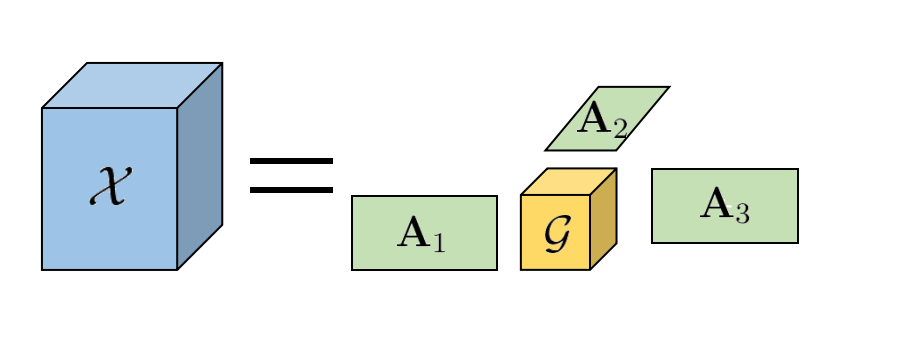
\includegraphics[width=0.6\textwidth]{figures/tucker_decomp.png}
    \caption{Tucker decomposition of a 3-dimensional tensor. Source:~\cite{tucker_decomp_pic}}
    \label{fig:tucker_decomp}
\end{figure}
Given a tensor $\boldsymbol{X} \in \mathbb{R}^{I_1 \times I_2 \times \dots \times I_N}$ and a matrix $\boldsymbol{A} \in \mathbb{R}^{J \times I_k}$, their $k$-mode product is written as: $$\boldsymbol{Y} = \boldsymbol{X} \times_k \boldsymbol{A}.$$ The tensor $\boldsymbol{Y} \in \mathbb{R}^{I_1 \times \dots \times I_{k-1} \times J \times I_{k+1} \times \dots \times I_N}$ contains elements: $$y_{i_J \dots i_{k-1} i_j i_{k+1} \dots i_N} = \sum_{i_k = 1}^{I_k} x_{i_1 i_2 \dots i_N} a_{j i_k}.$$ The core tensor $\boldsymbol{G}$ is usually much smaller than the original tensor $\boldsymbol{X}$. The algorithm takes $R$ as an argument, which defines the size of the core tensor $\boldsymbol{G}$.

The Tucker ALS algorithm uses SVD of different modes to create a tensor of a smaller size. Each iteration, the approximated tensor is created, and the error from the original one is calculated. When the convergence criterion is fulfilled or the maximum number of iterations is reached, the algorithm is stopped~\cite{tucker_decomp}.

On the other hand, the \textbf{CP ALS} algorithm decomposes the given tensor into the canonical polyadic (CP) decomposition with alternating least square method. The polyadic decomposition approximates a tensor $\boldsymbol{T}$ as a sum of $R$ rank-one tensors. For the smallest $R$, such that the equation holds, it is called the canonical polyadic decomposition. Let $\boldsymbol{T} \in \mathbb{R}^{I_1 \times I_2 \times \dots \times I_N}$ be a tensor of order $N$. The canonical polyadic decomposition of $\boldsymbol{T}$ is then written as: $$\boldsymbol{T} = \sum_{r = 1}^R a_1^{(1)} \otimes a_1^{(2)} \otimes \dots \otimes a_1^{(N)},$$ where $\boldsymbol{A} \in \mathbb{R}^{I_n \times R}$ are factor matrices with $r$-th column written as $a_r^{(n)}$, and $\otimes$ is the outer product. The decomposition of a 3-dimensional tensor can be seen in Figure \ref{fig:cp_decomp}.
\begin{figure}[h]
    \centering
    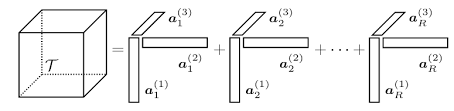
\includegraphics[width=0.8\textwidth]{figures/cp_decomp.png}
    \caption{Canonical polyadic decomposition of a 3rd-order tensor. Source: \cite{cp_decomp_pic}}
    \label{fig:cp_decomp}
\end{figure}
Let $\boldsymbol{A} \in \mathbb{R}^{I_1 \times I_2 \times \dots \times I_N}$ be an $N$-th-order tensor and $\boldsymbol{B} \in \mathbb{R}^{J_1 \times I_2 \times \dots \times J_M}$ be an $M$-th-order tensor. Then their outer product $\boldsymbol{A} \otimes \boldsymbol{B}$ is an $(M + N)$-th-order tensor and is defined as: $$(\boldsymbol{A} \otimes \boldsymbol{B})_{i_1 \dots i_N j_1 \dots j_M} = a_{i_1 \dots i_N} b_{j_1 \dots j_M}.$$ $R$ is a parameter of the algorithm that computes the canonical polyadic decomposition~\cite{cp_decomp}.

The CP ALS algorithm finds the factor matrices $\boldsymbol{A}_1, \boldsymbol{A}_2, \dots, \boldsymbol{A}_N$, which represent the CP decomposition. Each iteration, the factor matrices are updated one by one. To update a single factor matrix $\boldsymbol{A}_n$, the gradient of the least-squares objective function with respect to that matrix is calculated. Then, it is set to zero, and the factor matrix is found by solving the system of linear equations. The algorithm stops when the maximum number of iterations is reached or when the error between the original and approximated tensors is below the chosen threshold~\cite{cp_als}.

Moreover, \textbf{TNCP} solves the nuclear-norm regularized canonical polyadic tensor completion problem via the Alternating Direction Method of Multipliers (ADMM). Same as the CP ALS algorithm, it also finds the CP decomposition of the given tensor. In~\cite{tncp_rank_model}, the following model for tensor $\boldsymbol{T}$ completion problems has been proposed: $$\arg \min_{\boldsymbol{X}} \sum_{n = 1}^N w_n \rank(\boldsymbol{X}_{(n)}),$$ where $w_n$ are weights, $\boldsymbol{X}_{(n)}$ are the unfolded matrices along the n-th mode, and $\boldsymbol{X}_\Omega = \boldsymbol{T}_\Omega$, where $\Omega$ is a set of already filled values. In~\cite{tncp}, it has been proven that: $$\rank(\boldsymbol{X}_{(n)}) \leq \rank(\boldsymbol{A}_n),$$ where $A_n$ are the factor matrices of the CP decomposition of tensor $\boldsymbol{X}$. They updated the model as follows: $$\arg \min_{\boldsymbol{X}, \boldsymbol{U_n}} \sum_{n = 1}^N w_n \rank(\boldsymbol{A}_n),$$ where $\boldsymbol{X} = A_1 \otimes A_2 \otimes \dots \otimes A_N$, $\boldsymbol{X}_\Omega = \boldsymbol{T}_\Omega$, $A_n$  are the factor matrices of the CP decomposition of tensor $\boldsymbol{X}$, and $\otimes$ is the outer product. They relaxed the model into: $$\arg \min_{\boldsymbol{X}, \boldsymbol{A_n}} \sum_{n = 1}^N w_n ||\boldsymbol{A}_n||_{\textasteriskcentered},$$ where $\boldsymbol{X} = A_1 \otimes A_2 \otimes \dots \otimes A_N$, $\boldsymbol{X}_\Omega = \boldsymbol{T}_\Omega$, and $||\boldsymbol{A}_n||_{\textasteriskcentered}$ means the nuclear norm of the matrix $\boldsymbol{A}_n$, which is the sum of its singular values. The model can be reformulated as: $$\arg \min_{\boldsymbol{X}, \boldsymbol{A_n}} \sum_{n = 1}^N w_n ||\boldsymbol{A}_n||_{\textasteriskcentered} + \frac{\lambda}{2} ||\boldsymbol{X} - A_1 \otimes A_2 \otimes \dots \otimes A_N||_F^2,$$ where $\lambda$ is a regularization parameter and $||\boldsymbol{X}||_F^2$ is the Frobenius norm. 

This problem is solved with ADMM, which forms the partial augmented Lagrangian function with auxiliary variables $M_1, M_2, \dots, M_N$. Each iteration updates $M_n$ and $A_n$ one by one, and then $\boldsymbol{X}$ is updated. When the convergence criterion is fulfilled or the maximum number of iterations is reached, the algorithm stops.

In~\cite{silrtc} from 2012, the Simple Low Rank Tensor Completion (SiLRTC) algorithm was presented. Similar to~\cite{tncp}, they solve the following model: $$\arg \min_{\boldsymbol{X}} \sum_{n=1}^N w_n ||\boldsymbol{X}_{(n)}||_{\textasteriskcentered},$$ where $\boldsymbol{X}_\Omega = \boldsymbol{T}_\Omega$. The terms of this model cannot be solved independently. To face this problem, they introduced additional matrices $M_1, M_2, \dots, M_N$ and created the equivalent formulation: $$\arg \min_{\boldsymbol{X}, \boldsymbol{M}_n} \sum_{n=1}^N w_n ||\boldsymbol{M}_n||_{\textasteriskcentered},$$ where $\boldsymbol{X}_{(n)} = \boldsymbol{M}_n$ and $\boldsymbol{X}_\Omega = \boldsymbol{T}_\Omega$. They relaxed the constraints $\boldsymbol{X}_{(n)} = \boldsymbol{M}_n$ into $||\boldsymbol{X}_{(n)} - \boldsymbol{M}_n||_F \le d_n$, where $d_n$ is a threshold. For positive values of $\beta_n$, the model can be reformulated into: $$\arg \min_{\boldsymbol{X}, \boldsymbol{M}_n} \sum_{n=1}^N w_n ||\boldsymbol{M}_n||_{\textasteriskcentered} + \frac{\beta_n}{2}||\boldsymbol{X}_{(n)} - \boldsymbol{M}_n||_F^2,$$ where $\boldsymbol{X}_\Omega = \boldsymbol{T}_\Omega$.

Finally, the \textbf{SiLRTC} algorithm always optimizes one variable while the other variables are fixed. Variables $M_n$ are computed as: $$M_n = \boldsymbol{D}_\tau (\boldsymbol{X}_{(n)}),$$ where $\tau = \frac{w_n}{\beta_n}$ and $\boldsymbol{D}_\tau (\boldsymbol{X}_{(n)}) = \boldsymbol{U} \boldsymbol{\Sigma}_\tau \boldsymbol{V}^T$. Variable $\boldsymbol{X}$ is computed as: $$\boldsymbol{X}_{i_1 i_2 \dots i_N} = \left(\frac{\sum_n \beta_n \fold_n(\boldsymbol{M}_n)}{\sum_n \beta_n}\right)_{i_1 i_2 \dots i_N}$$ for the elements that are not in $\Omega$, and where $\fold_k(\boldsymbol{X}_{(k)}) = \boldsymbol{X}$. Each iteration updates variables $M_1, M_2, \dots, M_N$ one by one, and then variable $\boldsymbol{X}$ is updated. The algorithm stops when the maximum number of iterations is reached or when the error between the original and approximated tensors is within the chosen tolerance.

%---------------------------------------------------------------
\chapter{Model}
%---------------------------------------------------------------

Collaborative filtering methods are widely used in recommendation systems, where they predict a user's preference for a specific item. Similarly, these techniques can be leveraged to model football predictions by analyzing the historical results of matches between teams. The goal is to predict future match outcomes based on the observed interactions between home and away teams. My model stores the interactions between home and away teams in the form of match results, which are represented in a three-dimensional tensor. This chapter describes how I modeled football prediction as tensor completion.

\section{Tensor Completion for Football Prediction}
\label{model}
As I described in Section \ref{matrix_fac}, in recommender systems, interactions between users and items are stored. In my model, the interactions between teams are stored in the form of the results of the matches. To analyze more than a single season for the prediction, I used a tensor instead of a matrix.

Let $T \in \mathbb{R}^{n \times n \times s}$ be a tensor, where $s$ is the number of seasons and $n$ is the number of teams that played in all $s$ seasons. Then the number in the $i$-th row, $j$-th column, and $k$-th slice represents the result of the match between team $i$ and $j$ in the $k$-th season, where team $i$ was the home team and team $j$ played as the away team. Of course, a team cannot play against itself, so the elements on the diagonal of each slice are undefined. Also, the playing teams change throughout the years. Note that frequently, there are around twenty teams playing each season (depending on the league, there can be more or less). However, there are around fifty teams that played in all the used seasons in total, and the exact number will depend on the observed league. Hence, in each slice, only elements corresponding to the teams that played in the corresponding season are defined. It can be seen, therefore, that most of the elements of the tensor are undefined. These elements are not replaced with any number. They stay undefined, and in this way, they don't affect the prediction. The entries are represented as either a home-win (represented as 1), a home-loss (i.e., a win for the away team, represented as -1), or a draw (represented as 0).

I use the model to predict the second half of the last observed season. The results of all previous seasons' matches are known, as well as the results of the first half of the last season. Elements corresponding to the unplayed matches - the second half of the last season - are undefined. An illustration of a tensor can be seen in Figure~\ref{fig:tensor}. The blue elements represent the unplayed matches, which will be predicted. This partly filled 3D tensor is the input of my model.

\begin{figure}[h]
    \centering
    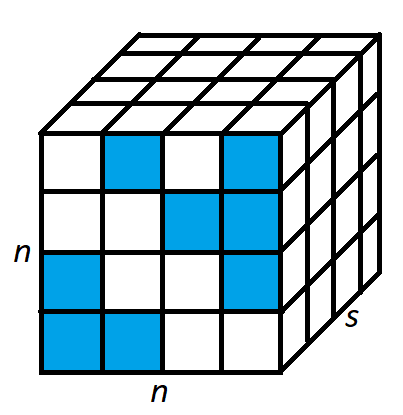
\includegraphics[width=0.3\textwidth]{figures/tensor1.PNG}
    \caption{Partly filled tensor representing the results}
    \label{fig:tensor}
\end{figure}

A tensor completion algorithm is used to complete the whole tensor. After completion, all the elements of the tensor are defined. As discussed in Section \ref{tensor_algs}, the algorithms usually decompose the tensor into more low-rank tensors, and by multiplying them, the fulfilled tensor is obtained. The rank $R \in \mathbb{N}$ of the low-rank tensors is a hyperparameter of the algorithm. Some of the defined elements of the original tensor can vary a little from the values in the fulfilled one. However, the goal of the algorithm is to make these differences as small as possible, so with enough iterations of the algorithm, they are insignificant. That is, the learning procedure is able to learn the training set accurately.

The fulfilled tensor returned by the algorithm consists of real numbers in comparison to the original one, which consisted only of 1, -1, 0, and undefined elements. These real numbers (at least those corresponding to the predicted matches) need to be turned into numbers only from the set \{1, -1, 0\}. For this purpose, a threshold $t$ is used. Let $t \in \mathbb{R}$ be a real number from the interval [0, 0.25]. Then, the number $f(x)$ after applying the threshold to number $x$ can be defined as:
\[   
f(x) = 
     \begin{cases}
       1 &\quad\text{if } x\ge 0 + t\\
       -1 &\quad\text{if } x\le 0 - t\\
       0 &\quad\text{otherwise.}\\
     \end{cases}
\]
The threshold is a hyperparameter, and I found the best value for it for each league, as I described in Section \ref{hyperparameters}. The closer the threshold is to 0, the fewer draws the model predicts. If $t = 0$, the model doesn't predict draws at all. On the other hand, if the threshold is too high, draws are predicted too often, which is a problem considering that only about 25\% of games end in a draw. This is why finding the right value for $t$ is crucial for the model to work properly.

After applying the threshold, the prediction is extracted. If the element corresponding to the predicted match is equal to 1, the model predicts the home team's win. If it is -1, the model predicts the away team's win, and if it is equal to 0, the model predicts a draw. The diagram of the whole algorithm is shown in Figure~\ref{fig:diagram}.

\begin{figure}[h]
    \centering
    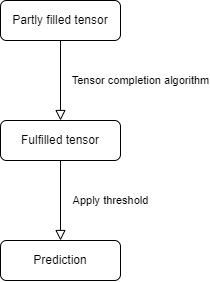
\includegraphics[width=0.3\textwidth]{figures/diagram.png}
    \caption{Football prediction with the tensor completion algorithm}
    \label{fig:diagram}
\end{figure}

%\section{Using SVD to improve other methods accuracy}
\section{Extracting Tensor Completion Embeddings for Football Prediction}
\label{embeddings}

There is information about how each team plays as the home team and as the away team in the tensor. More precisely, this information is available for each season. Each slice of the tensor corresponds to one season, so it is possible to extract this information. I extracted this information from the last slice that corresponds to the season that I aim to predict. Using SVD, I obtained the information in the form of feature vectors.

Let $\boldsymbol{A} \in \mathbb{R}^{m \times n}$ be a matrix with rank $r$. Then, orthogonal matrices $\boldsymbol{V} \in \mathbb{R}^{n \times n}$ and $\boldsymbol{U} \in \mathbb{R}^{m \times m}$, and a diagonal matrix $\boldsymbol{\Sigma} \in \mathbb{R}^{m, n}$ with positive numbers $\sigma_1 \ge \sigma_2 \ge \dots \ge \sigma_r$ on the diagonal, satisfy the following equation:
$$\boldsymbol{A} = \boldsymbol{U} \boldsymbol{\Sigma} \boldsymbol{V}^T,$$
which is called singular value decomposition (SVD). The representation of SVD is shown in Figure~\ref{fig:svd}. The numbers $\sigma_1, \sigma_2, \dots, \sigma_r$ are the singular values of matrix $\boldsymbol{A}$, which are square roots of eigenvalues of matrices $\boldsymbol{A}^T \boldsymbol{A}$ and $\boldsymbol{A} \boldsymbol{A}^T$. The columns of matrices $\boldsymbol{V}$ and $\boldsymbol{U}$ are the corresponding eigenvectors forming an orthonormal basis~\cite{svd}.

\begin{figure}[h]
    \centering
    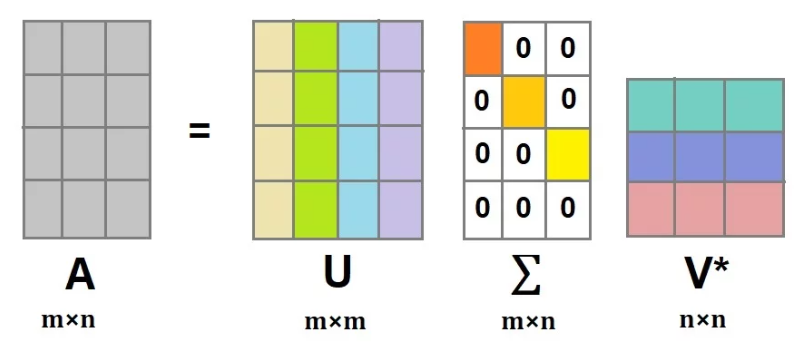
\includegraphics[width=0.6\textwidth]{figures/svd.PNG}
    \caption{Representation of SVD. Source:~\cite{svd_pic}}
    \label{fig:svd}
\end{figure}

I used singular value decomposition to obtain information on how each team plays in home matches and in away matches during the last season. Firstly, I used the tensor completion algorithm to fill the entire tensor. This way, there was an interaction for each game of the last season. For the first half of the season, it was the real result, and for the second half, it was a prediction. Let $\boldsymbol{M} \in \mathbb{R}^{n \times n}$ be the last slice of the tensor representing the last season. I performed SVD of this matrix $\boldsymbol{M}$, getting three matrices $\boldsymbol{U}, \boldsymbol{V}, \boldsymbol{\Sigma} \in \mathbb{R}^{n \times n}$. Then, I defined the home feature matrix $\boldsymbol{H} \in \mathbb{R}^{n \times n}$ and the away feature matrix $\boldsymbol{A} \in \mathbb{R}^{n, n}$ as follows:
$$\boldsymbol{H} = \sqrt{\boldsymbol{\Sigma}} \boldsymbol{V}^T$$
$$\boldsymbol{A} = \boldsymbol{U} \sqrt{\boldsymbol{\Sigma}}.$$
The rows of matrix $\boldsymbol{H}$ represent feature vectors, where each vector belongs to one team and represents how this team plays during the last season as the home team. The columns of matrix $\boldsymbol{A}$ represent feature vectors, which represent how the team plays as the away team. These feature vectors of length $n$ were then used to create new models. The whole algorithm for obtaining the feature vectors is described in Figure~\ref{fig:svd_diagram}. These models are based on the same machine learning algorithms as the baselines. In addition to the original features used in the baseline methods, the tensor completion embeddings represented by the feature vectors were included in the input of the model. The scheme of general model with the tensor completion embeddings is pictured in Figure \ref{fig:nn_vectors_diagram}.

\begin{figure}[h]
    \centering
    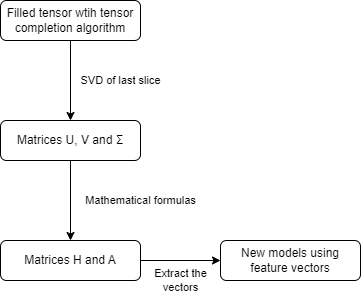
\includegraphics[width=0.5\textwidth]{figures/svd_diagram.png}
    \caption{Algorithm for extracting the feature vectors}
    \label{fig:svd_diagram}
\end{figure} 

\begin{figure}[h]
    \centering
    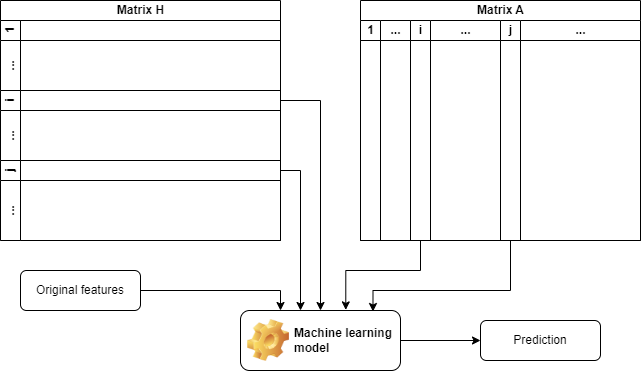
\includegraphics[width=1\textwidth]{figures/model_vectors.png}
    \caption{Machine learning model using tensor completion embeddings}
    \label{fig:nn_vectors_diagram}
\end{figure}

%---------------------------------------------------------------
\chapter{Experiments}
%---------------------------------------------------------------
This chapter discusses the experiments conducted in the thesis. Firstly, I will describe the datasets, conduct a statistical analysis, and provide information on the sources and feature selection process. Secondly, I will present and describe the baselines, followed by a description of the validation procedure and hyperparameter selection. Finally, I will discuss the results of our experiments.

Two distinct experimental approaches were undertaken:

\begin{itemize}
    \item I tested the effectiveness of tensor completion against baselines in a comparable scenario. This entailed providing the baselines with only the data that would typically be used in a tensor completion problem, such as the percentage of victories as a home team, the percentage of victories of an away team in past seasons, and so on;
    \item I evaluated the potential of combining tensor completion embeddings with traditional football prediction methods. Specifically, I provided these embeddings to individual football prediction methods and assessed whether the additional information could enhance their accuracy.
\end{itemize}

\section{Dataset}
\label{dataset}
Most of the countries in the world have their own football league. Nowadays, the most famous football leagues are from Europe. The \textit{English Premier League} (EPL), founded in 1888, holds the status of the oldest league in the world and is frequently considered to have the toughest competition. However, \textit{La Liga Primera División} (LLPD), the first football league in Spain, is also very prestigious due to the fact that Spanish teams frequently win international tournaments. Other famous European leagues include, for example, the \textit{German Bundesliga} (BL) or the \textit{Italian Serie A} (SA). 

Popular and historic football leagues also originate from South America. The \emph{Argentine Primera División}, a league from Argentina, is the oldest league on this continent, while the first professional Brazilian football league, called \textit{Brasileiro Série A} (BSA), was established in 1902. In most of the prestigious leagues in the world, twenty teams compete in a season. However, note that in Bundesliga, it is different, and there are only eighteen teams competing~\cite{leagues}.

Our dataset is composed of games from five leagues: (1) four prestigious European leagues: EPL, BL, LLPD, and SA; and (2) games of one league from South America: BSA. In this way, I could analyze the behavior of our method in a league outside the European continent. The data is based on results and statistics of matches and was gathered from Football-Data.co.uk~\cite{football_data}. Match results and statistics for each season of a league are stored in a CSV file. For the European leagues, the data is available from the 1993/94 season, and for each match of the season, there are several pieces of side information saved, such as the date of the match, names of the teams, the result, and statistics from the game itself, such as the number of goals, shots, corner kicks, and fouls (all for both teams). On the other hand, for the Brazilian league, the available data consists of seasons from 2012. Note that, for the Brazilian league, also fewer statistics are available. There is information about the result and the number of goals, but no more statistics (e.g., the number of corners of the away team) from the games. Betting data, although present in the dataset, is out of the scope of this research.

My study is limited to seasons prior to the coronavirus pandemic. During this period, there were minimal or no fans present at the games. Since fans play an essential role in football and contribute significantly to the home advantage, limiting the scope to this period will enable me to eliminate the pandemic's effects and gain a better understanding of how team competitiveness affects football prediction and how inter-season interference influences the prediction accuracy when using tensor completion. Therefore, I have gathered data only up to season 2018/19.

Additional statistics of the teams were gathered from the FIFA game, that are available on the website \textit{fifaindex.com}~\cite{fifa}. FIFA is a series of football simulators with real teams and players. For each team, there are attack, midfield, defense, and overall ratings. In the same line as~\cite{BPL_logistic_regression}, the attack and defense statistics were used. The FIFA game has different versions from 94 to 23. Since the statistics from the versions of the game from 05 are stored on the website, the ratings related to each season from the year 2005 till now were collected. However, note that the ratings were not achievable for all teams for some leagues in some seasons.

The statistics are saved back to 2005, so they cannot be gathered for the previous seasons. Models that use these ratings as features do not take into account data this old, so it was not a problem. The names of the teams were changing throughout the years, so this had to be taken into consideration. There are many more statistics for individual players on the website, but only the teams' ratings were focused on.

\subsection{Dataset Analysis}
\label{dataset_analysis}

To gain a deeper insight into the data and understand phenomena such as balancing the dataset, this section includes an analysis of the dataset to identify differences between leagues. The analysis focuses on percentages of home wins, draws, and away wins, as well as the distribution of goal differences in individual matches.

In the EPL, there were 46.22\% of home wins, 26.06\% of draws, and 27.73\% of away wins throughout the seasons 1993/94 to 2018/19, as can be seen in Figure~\ref{fig:epl_mr}. By analyzing the figure, it is clear that the home advantage is significant. Often, away wins occur slightly more than draws. However, in some seasons (e.g., 1998/1999), there were more draws than away wins, but in the last seasons, more matches ended as an away win than as a draw consistently. These results show that the dataset is slightly unbalanced.%, which makes the prediction task more difficult.
\begin{figure}[h]
    \centering
    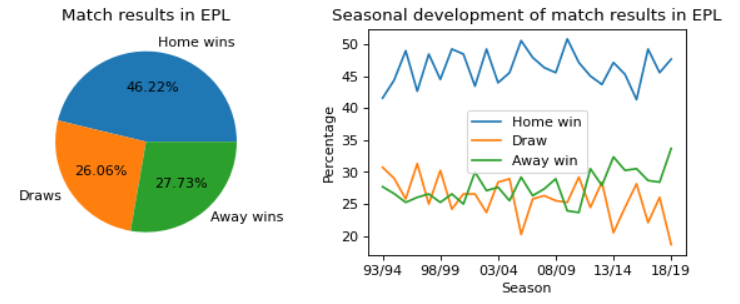
\includegraphics[width=1\textwidth]{figures/epl_subgraph.png}
    \caption{Overall statistic of match results and development of the match result percentages of EPL in seasons from 1993/94 to 2018/19.}
    \label{fig:epl_mr}
\end{figure}

Figure~\ref{fig:epl_gd} shows the distribution of goal differences in EPL matches from seasons 1993/94 to 2018/19. There were more games where the home team scored more goals than the away team (positive goal difference) than games where the away team scored more goals than the home team, which corresponds to the home advantage. The highest number of matches ended with a goal difference of zero, which agrees with the relatively high percentage of draws.
\begin{figure}[h]
    \centering
    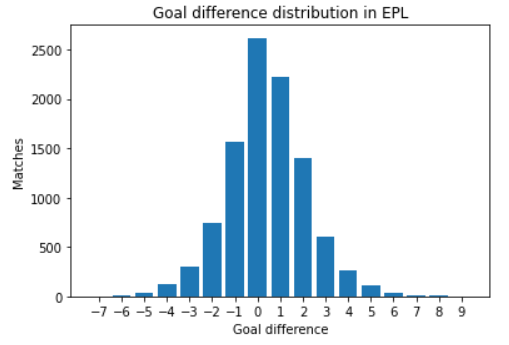
\includegraphics[width=0.7\textwidth]{figures/epl_gd.png}
    \caption{Distribution of goal differences of EPL matches from seasons 1993/94 to 2018/19.}
    \label{fig:epl_gd}
\end{figure}

In the other leagues (BL, LLPD, SA, and BSA), the percentages were similar as seen in Figures~\ref{fig:bl_mr},~\ref{fig:llpd_mr},~\ref{fig:sa_mr}, and~\ref{fig:bsa_mr}, respectively. The Italian and Brazilian leagues differ the most, as in both leagues, more matches ended with a draw than with an away win. Also, SA is the league with the most draws at 27.77\% (Figure~\ref{fig:sa_mr}), and BSA is the league with the most home wins at 48.61\% and the least draws at 24.33\% (Figure~\ref{fig:bsa_mr}). The developments throughout the years were similar as well. In the last few years, there have been more away wins than draws, with the exception of BSA (Figure~\ref{fig:bsa_mr}), where the number of draws consistently exceeds the number of away wins.
\begin{figure}[h]
    \centering
    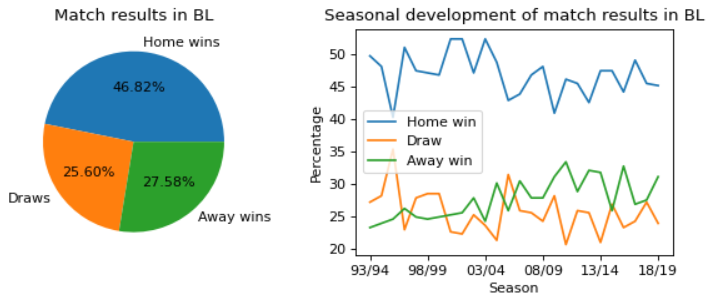
\includegraphics[width=1\textwidth]{figures/bl_subgraph.png}
    \caption{Overall statistic of match results and development of the match result percentages of BL in seasons from 1993/94 to 2018/19.}
    \label{fig:bl_mr}
\end{figure}
\begin{figure}[h]
    \centering
    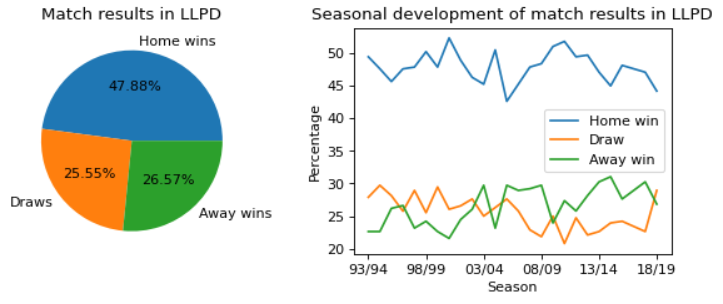
\includegraphics[width=1\textwidth]{figures/llpd_subgraph.png}
    \caption{Overall statistic of match results and development of the match result percentages of LLPD in seasons from 1993/94 to 2018/19.}
    \label{fig:llpd_mr}
\end{figure}
\begin{figure}[h]
    \centering
    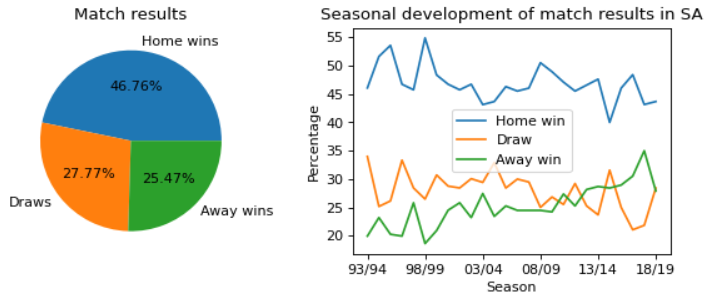
\includegraphics[width=1\textwidth]{figures/sa_subgraph.png}
    \caption{Overall statistic of match results and development of the match result percentages of SA in seasons from 1993/94 to 2018/19.}
    \label{fig:sa_mr}
\end{figure}
\begin{figure}[h]
    \centering
    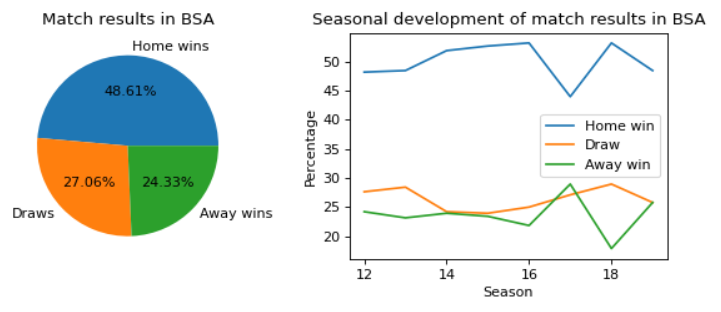
\includegraphics[width=1\textwidth]{figures/bsa_subgraph.png}
    \caption{Overall statistic of match results and development of the match result percentages of BSA in seasons from 1993/94 to 2018/19.}
    \label{fig:bsa_mr}
\end{figure}

The goal difference distributions of BL, LLPD, SA, and BSA, shown in Figures~\ref{fig:bl_gd},~\ref{fig:llpd_gd}, \ref{fig:sa_gd}, and~\ref{fig:bsa_gd} respectively, are very similar as well. There were always more games concluding with a positive goal difference than with a negative one. The most different league is BSA, where almost as many matches ended with a goal difference of one as there were draws (Figure~\ref{fig:bsa_gd}).  

\begin{figure}[h]
    \centering
    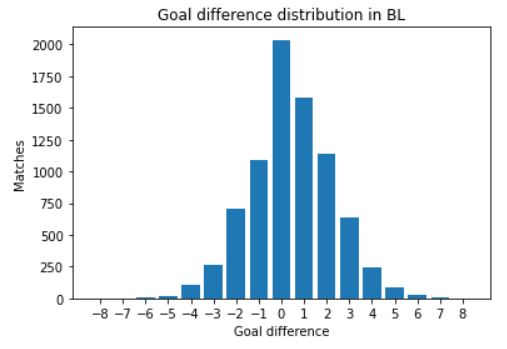
\includegraphics[width=0.7\textwidth]{figures/bl_gd.png}
    \caption{Distribution of goal differences of BL matches from seasons 1993/94 to 2018/19.}
    \label{fig:bl_gd}
\end{figure}
\begin{figure}[h]
    \centering
    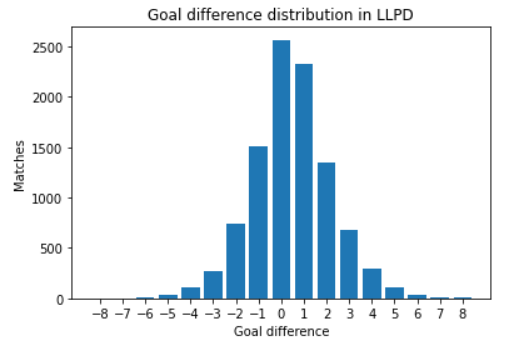
\includegraphics[width=0.7\textwidth]{figures/llpd_gd.png}
    \caption{Distribution of goal differences of LLPD matches from seasons 1993/94 to 2018/19.}
    \label{fig:llpd_gd}
\end{figure}
\begin{figure}[h]
    \centering
    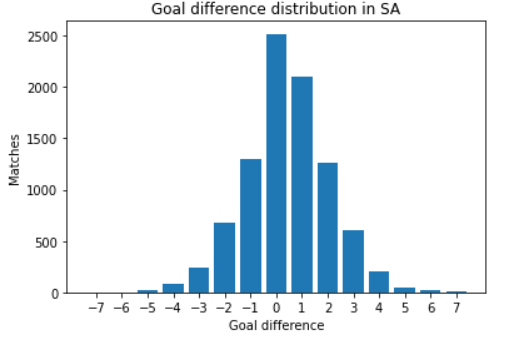
\includegraphics[width=0.7\textwidth]{figures/sa_gd.png}
    \caption{Distribution of goal differences of SA matches from seasons 1993/94 to 2018/19.}
    \label{fig:sa_gd}
\end{figure}
\begin{figure}[h]
    \centering
    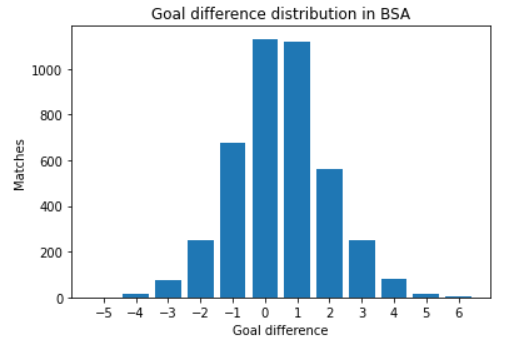
\includegraphics[width=0.7\textwidth]{figures/bsa_gd.png}
    \caption{Distribution of goal differences of BSA matches from seasons 1993/94 to 2018/19.}
    \label{fig:bsa_gd}
\end{figure}
 


\subsection{Features}
Different models in the literature use different feature sets, but some of the features are the same and some of them are similar. I gathered all the necessary features for all baselines and models from the achieved data. The match results are represented as integers: 1 for a home win, 0 for a draw, and -1 for an away win. Several of our baselines and further models used the average number of goals in the current season for each team as features. I calculated these numbers from the game statistics. The same was done with shots, corner kicks, and fouls. The percentages of wins, losses, and draws in the current season were also often applied, sometimes percentages of earlier encounters as well. Also, results of the five previous matches or the current streak were added to the feature sets. Often, the ratings from the FIFA game were used as well. Information about the number of days from the previous match and if the team was in a lower league last year were also applied. Sometimes the betting odds for a home win, an away win, and a draw were used, as well as the average number of goals in the last five matches.

My model, which relies only on tensor completion, cannot use any of the in-game statistics or additional information. To compare this model better to the baselines, I have computed a feature set which consists only of features extracted from game results. In this work, we refer this computed features by  \textit{Win-loss} feature set. These features form a subset of the above-mentioned ones. They are percentages of wins, losses, and draws in the current season and from earlier encounters. The percentages from only home and only away matches are also added. Note that, they are equivalent information when compared to those ones used in the tensor completion method.

\section{Baselines}
\label{baselines}

To cover a diverse range of machine learning techniques utilized in football prediction literature, I carefully selected three popular models: Logistic Regression, PCA-based Naive Bayes, and Artificial Neural Network. In addition, as a natural baseline, I employed matrix factorization, which has previously been applied to predict basketball outcomes in related work~\cite{NBA_matrix_factorization}.

As previously mentioned, two experimental strands were considered. Our experimental approach involved two stages. Firstly, I compared the effectiveness of tensor completion against baselines in a comparable scenario, which involved providing the baselines with only the data typically used in a tensor completion problem.

Secondly, I explored the potential of incorporating tensor completion embeddings with traditional football prediction methods. To this end, I provided these embeddings to individual football prediction methods and evaluated whether the additional information could boost their predictive accuracy. For this purpose, I kept the procedures as similar as possible to those described in the original paper. In the following sections, I will describe the features and further details.

\subsection{Logistic Regression}
\label{lr}
I chose a model based on Logistic Regression described in~\cite{BPL_logistic_regression} as one of the baselines. In this implementation, only the ratings from the FIFA game were fed into the model as features, specifically home offense, home defence, away offense, and away defence. The data is available online as described in~\cite{BPL_logistic_regression}. In certain seasons and leagues, I encountered instances of missing ratings for a few teams. Given that ratings were the only available features, I opted against imputing the missing values. Instead, I leveraged data from other seasons where ratings for all teams were available for training purposes. In the case of the Brazilian league, numerous teams were found to have missing data each season. Consequently, I decided to exclude these features altogether. In this league, we only utilized the Win-loss feature set for our model.

In the original paper, the authors experimented with the amount of training data, and the best results were achieved with five training seasons. To keep the model as similar as possible, I created a training dataset from five seasons as well. Thus, I used seasons 2012/13 to 2016/17 for training, season 2017/18 for validation, and season 2018/19 for testing.

The authors did not mention how they dealt with draws. It is reasonable to assume that they ignored matches that ended in a draw. However, I needed to compare this baseline approach to other models that can predict draws, so I modified the Logistic Regression model to also predict draws. During training, I excluded draw games because Logistic Regression cannot learn to classify into three classes. However, I included draw games during validation and testing. Since Logistic Regression always returns a value between 0 and 1, I represented wins as 1 and away wins as 0. To predict draws, I defined a modifiable hyperparameter threshold $t$. If the returned value is lower than $0.5 - t$, an away win is predicted; if it is higher than $0.5 + t$, a home win is predicted, and a draw is predicted otherwise. During the validation phase, I experimented with different threshold values and chose the one with the highest accuracy on the validation dataset. Finally, I evaluated the baseline on the testing dataset with the chosen threshold.

\subsection{Naive Bayes with PCA}
In~\cite{Dutch_football}, the authors applied many machine learning algorithms for predicting the football results. The highest accuracy for the public data was achieved by the model based on Naive Bayes using PCA with three components as a dimensionality reduction technique (tied for the first place with ANN). 

In the original paper, the features were divided into three feature sets: public data feature set, betting odds feature set, and hybrid feature set. I chose to implement the public feature set, as it constituted the primary feature set. There are 32 features in the public feature set, which are further divided into features for both teams, features for the home team, features for the away team, and features for the combination of home and away team.

More specifically, there are numerous features retrieved for both teams, such as percentages of wins, draws, and losses this season, average scored and conceded goals this season, or number of days since the previous match. Some features, such as the number of matches coached by the current coach or average goals by top-scorer, were not accessible, so I replaced them with, for example, the average fired and conceded shots, to keep the number of features as similar as possible. For the home team, there are percentages of wins, draws, and losses in home matches, and for the away team, the same percentages are calculated but for away matches. Percentages of earlier encounters are gathered for the combination of the home and away team, specifically percentages of results of the earlier encounters on the same ground and on both grounds: win by the home team, draw, and win by the away team.

The authors used thirteen seasons, and they formally stated that more data would have negative consequences. In the same spirit, I gathered data from thirteen seasons as well. I used seasons 2006/07 to 2016/17 for training, season 2017/18 for validation, and season 2018/19 for testing. I also kept hyperparameterization and split train-test as in~\cite{Dutch_football}.

Moreover, in the source work, PCA with three components and Naive Bayes were used for prediction. The authors did not specify certain details regarding the Naive Bayes implementation. I used Gaussian Naive Bayes because it is the most common implementation.

\subsection{ANN}

ANN is one of the most used and accurate methods to predict football outcomes. As a baseline, I implemented ANN according to ~\cite{BPL_ANN_logistic_regression}.

As features, the authors gathered, for example, the average number of goals, betting odds on win, attack strength, or streak as features. For attack strength, I used stats from the FIFA game obtained by the same procedure as described in Section~\ref{lr}. For streak, I retrieved the results from previous matches and implemented the feature as the current number of consecutive wins or losses. I wasn't able to gather features like players’ performance index or managers’ win. I replaced these features, for instance, with the average number of fouls or number of days since the last match.

The authors applied only the 2014/15 season for training. To follow a similar pattern, season 2016/17 was for training, 2017/18 for validation, and 2018/19 for testing. Thus, I keep the validation and testing datasets the same as in other baselines and models. I didn't need the validation data for hyperparameter setting, but it was used for selecting the best checkpoint of the training - the number of epochs.

There is a lack of information regarding the details of the architecture of the ANN. Thus, I created a Neural Network with three dense layers with 64, 32, and 16 neurons. After each layer, I applied dropout of 0.2 to overcome overfitting. The dense layers use ReLU activation function because it is a standard choice. The output layer consists of three neurons with softmax activation function because the task is 3-class classification. As the loss function serves categorical cross-entropy, which is suitable for categorical classification, and as the optimizer was picked Adam, since it is the most robust optimizer for dense Neural Networks. I always let the model train for a hundred epochs, after each a checkpoint was made, and the best one was chosen according to the validation accuracy. How exactly the network was evaluated on the testing dataset is described in section~\ref{eval_proc}.

\subsection{Matrix Factorization}
In~\cite{NBA_matrix_factorization}, matrix factorization was applied to predict basketball results, but the authors did not specify how the matrix was factorized or how missing values were filled. Predicting basketball outcomes differs from predicting football results due to differences in the pace of the game and the probability of draws. To predict football outcomes, I adapted a matrix factorization model from this work. The matrix represents a single season, with each element representing a match and each row and column representing the participating teams. However, this implementation cannot handle negative numbers, so instead, we used 1 to denote a home win, 2 for a draw, and 3 for an away win. This allows us to maintain the intensity of the results. The method used to train the matrix factorization model is based on stochastic gradient descent~\cite{mf_impl}.

The matrix factorization model is always trained and executed on only one matrix, so the amount of training data is not a factor. I used the second half of the 2017/18 season for validation and the second half of the 2018/19 season for testing.

There is a hyperparameter $K$, which indicates the number of dimensions of the latent vectors. Additionally, a threshold $t$ needs to be applied to define when a draw is predicted. Let $t \in \mathbb{R}$ be a real number from the interval [0, 0.25]. If the filled value is smaller than $2 - t$, a home win is predicted. If it is greater than $2 + t$, an away win is predicted. Otherwise, a draw is predicted. Hyperparameters $K$ and $t$ are experimented with, and the values with the highest validation accuracy are chosen. The model is then evaluated on the testing season using these values.

\section{Evaluation Procedure}
\label{eval_proc}
Cross-validation is not suitable for this task because the data has a chronological order. In practice, machine learning models cannot learn from matches that have not yet been played, which would be the case in cross-validation~\cite{Dutch_football}. Instead, to evaluate each match, I considered only training data from games that happened before the match being evaluated.

To maximize the amount of training data for each match as much as possible, the testing dataset was split into slices. Each slice corresponds to approximately one round of the league. Due to other tournaments, some matches are often delayed, and some games from the previous round are played later than games from the next round. To address this issue, I always took the number of matches that should be in a round and added the ones that were played on the same day as the last one. This way, I sometimes had bigger slices than one round, but the chronological order was kept. For evaluating each slice, the training dataset and all the previous slices were considered as training data. In other words, the slices were evaluated chronologically, and after evaluating, the slice was added to the training data. The process can be seen in Figure \ref{fig:eval}. With this approach, for each round, the model was trained on all the data available at that moment.
\begin{figure}[h]
    \centering
    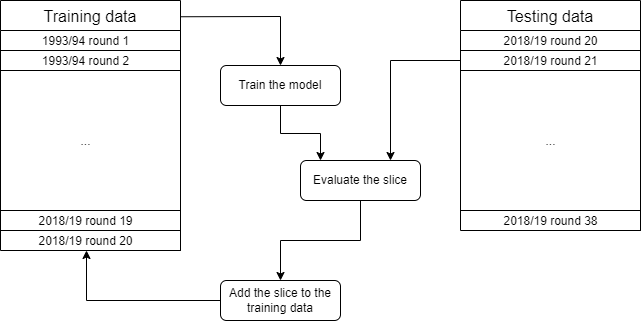
\includegraphics[width=0.9\textwidth]{figures/eval.png}
    \caption{One step of the evaluation procedure - the model is trained on the current training data, the testing slice is evaluated and added to the training data.}
    \label{fig:eval}
\end{figure}

To have some data to train on from the current season, only the second half of the testing season was used as the testing dataset, and the first half was added to the training data. The evaluation was done exactly the same way for each league and for each model and baseline to make them comparable.

\section{Hyperparameter Selection}
\label{hyperparameters}
Here I will mention some implementation details and how the hyperparameters were selected. All available data was used for training, meaning seasons from 1993/94 to the first half of the season 2017/18 and the second half of the 2017/18 season served as the validation dataset. For testing, the model was trained on all data from seasons 1993/94 to the first half of the season 2018/19 and evaluated on the second half of this season, meaning the testing dataset was the second half of the 2018/19 season. A tensor was created that represents the results from all the seasons.

One of the hyperparameters of all tensor completion algorithms is the maximum number of iterations. This hyperparameter defines how long the algorithm runs and can have a significant impact on how well it converges. I experimented with different numbers of iterations ranging from 10 to 5000. For each number of iterations, I fixed the other hyperparameters and ran the algorithm twenty times and observed the variance of the validation accuracy of the individual runs, which was the criterion. The average accuracy was stable, so I chose the maximum number of iterations where the runs had the smallest variance, indicating that the algorithm converged the best.

For all tensor completion algorithm I applied the threshold, described in Section \ref{model}, as a hyperparameter. This hyperparameter defines how often a draw is predicted, and eleven values from the interval [0, 0.25] were tested. Another hyperparameter is $R$, which defines the size of the decomposition. The best hyperparameters for each algorithm were chosen according to the validation accuracy of the EPL. TNCP achieved the best accuracy, so it was applied on all leagues, and its hyperparameters were optimized for each league individually. The model was evaluated with TNCP algorithm and chosen hyperparameters on the testing dataset in the end.

\section{Tensor Completion Embeddings}
\label{vectors}
As described in Section \ref{embeddings}, I extracted feature vectors from the last season using tensor completion and SVD. With these vectors, I compared the models based on the same algorithms as the baselines with and without the vectors. I added the feature vectors to the inputs of the model, saved the $H$ and $A$ matrices, and for each match, I loaded the vectors corresponding to the playing teams. The best results with the feature vectors were achieved by ANN, so I experimented more with this model. I changed two aspects: I experimented whether it's better to do the SVD before or after applying the threshold in the tensor completion algorithm, and I observed whether it helps to add away feature vector to the home team and home feature vector to the away team. In total, I applied four options covering all the combinations. These experiments are discussed more in Section \ref{improving}.

\section{Results}

\subsection{Comparison of Tensor Completion Model with Baselines}
The results for all leagues for the Win-loss feature set, which consists only of features gathered from game results, can be found in Table~\ref{table:win_loss}. The matrix factorization and tensor completion models can be compared with the baselines using this feature set. The last column shows the accuracy achieved by always predicting the win of the home team. In EPL and BSA had the tensor completion algorithm the best results. In BL, the highest accuracy was achieved by PCA + NB, in LLPD by PCA + NB and TC, and in SA by ANN. The tensor completion algorithm was the best method in three out of five leagues and in the other two it took second place, while being very close to the first place. These results support the idea, that tensor completion can analyse matches from previous seasons better than other models.

\noindent \textbf{REMARK:} All machine learning techniques beat the trivial strategy of always predicting the home team to win. The worst results were obtained in BSA compared to the trivial strategy, with only the tensor completion algorithm equalling it. This possibly can be attributed to the lack of data and the fact that the percentage in the testing dataset was 2\% higher than the average.

\begin{table}
\begin{center}
\begin{tabular}{|p{0.15 \textwidth}| l | p{0.1 \textwidth} | l | l | l | l |}
 \hline
 Win-loss & LR & PCA + NB & ANN & MF & TC & Home \\ 
 \hline
 EPL & 55.26\% & 54.74\% & 55.26\% & 45.79\% & $\mathbf{56.32\%}$ & 45.26\% \\  
 \hline
 BL & 49.02\% & $\mathbf{50.98\%}$ & 46.41\% & 44.44\% & 50.33\% & 45.1\% \\ 
 \hline
 LLPD & 45.26\% & $\mathbf{50.53\%}$ & 48.95\% & 41.05\% & $\mathbf{50.53\%}$ & 40\% \\  
 \hline
 SA & 45.26\% & 46.84\% & $\mathbf{47.89\%}$ & 43.16\% & 47.37\% & 43.68\% \\ 
 \hline
 BSA & 46.32\% & 46.32\% & 47.37\% & 43.16\% & $\mathbf{50.53\%}$ & $\mathbf{50.53\%}$ \\  
 \hline
\end{tabular}
\caption{Accuracy of different models and baselines on the Win-loss feature set}
\label{table:win_loss}
\end{center}
\end{table}

In Figure~\ref{fig:cm_epl}, the confusion matrix of the tensor completion model on the EPL dataset is presented. The confusion matrix only includes the testing split of the dataset - the second half of the 2018/19 season. Home wins are predicted well, and away wins are also decent, but draws are predicted poorly, with less than half of them being correctly predicted.

Confusion matrices for BL, LLPD, SA, and BSA can be seen in Figures~\ref{fig:cm_bl},~\ref{fig:cm_bllpd},~\ref{fig:cm_sa}, and~\ref{fig:cm_bsa}, respectively. Home wins have good prediction accuracy, but draws are poorly predicted in all leagues. Away wins are predicted well in LLPD with more than half of them being correctly predicted, and decently in SA with an accuracy of over 40\%. In other leagues, they are predicted poorly.

\begin{figure}[h]
    \centering
    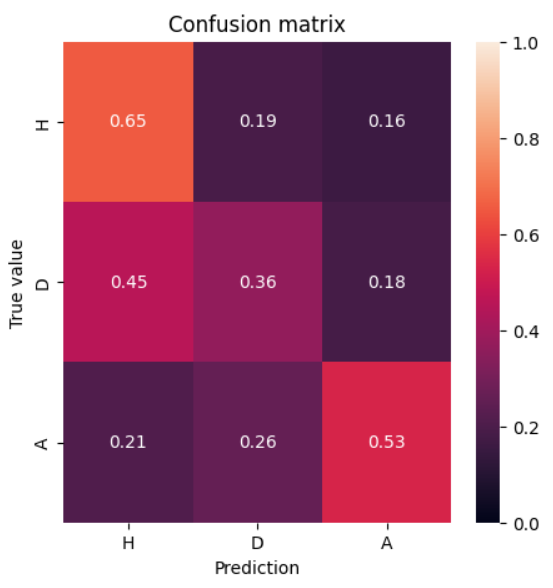
\includegraphics[width=0.6\textwidth]{figures/cm_epl.png}
    \caption{Confusion matrix of the tensor completion model evaluated on testing dataset of EPL.}
    \label{fig:cm_epl}
\end{figure}

\begin{figure}[h]
    \centering
    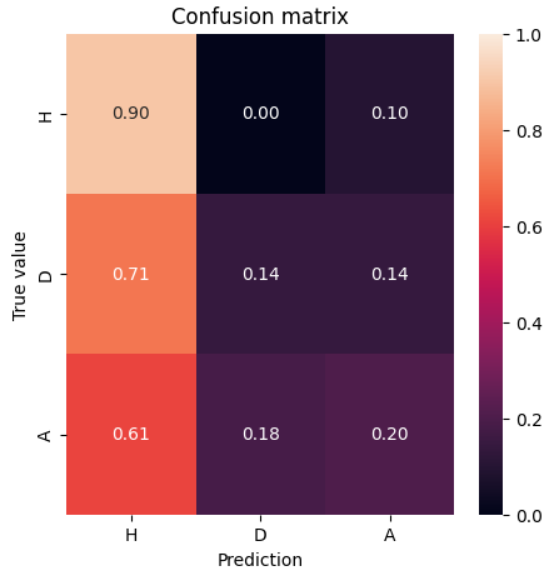
\includegraphics[width=0.6\textwidth]{figures/cm_bl.png}
    \caption{Confusion matrix of the tensor completion model evaluated on testing dataset of BL.}
    \label{fig:cm_bl}
\end{figure}

\begin{figure}[h]
    \centering
    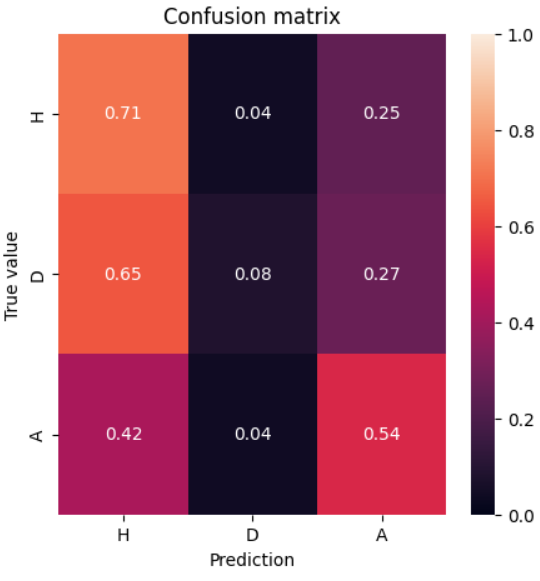
\includegraphics[width=0.6\textwidth]{figures/cm_llpd.png}
    \caption{Confusion matrix of the tensor completion model evaluated on testing dataset of LLPD.}
    \label{fig:cm_bllpd}
\end{figure}

\begin{figure}[h]
    \centering
    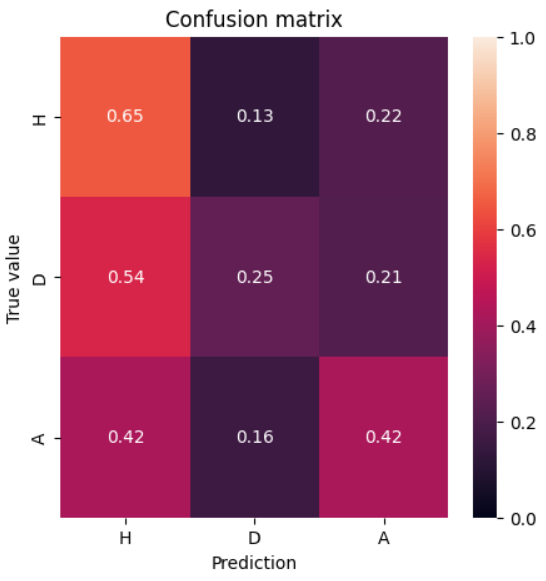
\includegraphics[width=0.6\textwidth]{figures/cm_sa.png}
    \caption{Confusion matrix of the tensor completion model evaluated on testing dataset of SA.}
    \label{fig:cm_sa}
\end{figure}

\begin{figure}[h]
    \centering
    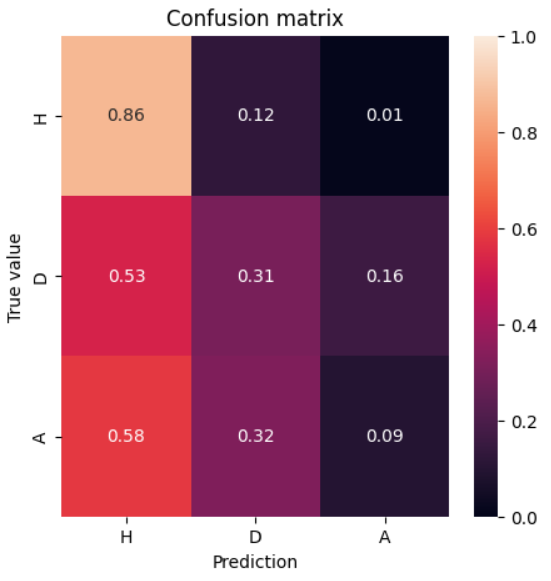
\includegraphics[width=0.6\textwidth]{figures/cm_bsa.png}
    \caption{Confusion matrix of the tensor completion model evaluated on testing dataset of BSA.}
    \label{fig:cm_bsa}
\end{figure}

\subsection{Improving the Accuracy by Adding Tensor Completion Embeddings}
\label{improving}
In this section, we will analyse the behaviour of methods used in the baselines by adding the feature vectors to their inputs. In Table~\ref{table:epl}, the test accuracy of models and baselines on the EPL dataset with other feature sets can be seen. The first row shows the accuracy of the baselines with the original features as described in the papers. In the second row, the combination of the Original and Win-loss feature sets was used, and in the third row, the feature vectors representing tensor completion embeddings were added. The baseline based on PCA and Naive Bayes already includes the Win-loss feature set in the Original one, so I did not consider the Original + Win-loss feature set for this baseline.

The accuracy of the models based on LR and ANN increased by more than 2\% when the feature vectors were added to the inputs. However, adding these vectors did not increase the accuracy of the other models applied in the baselines.

\begin{table}
\begin{center}
\begin{tabular}{|p{0.15 \textwidth}| l | p{0.1 \textwidth} | l | l | l | l |}
 \hline
 EPL & LR & PCA + NB & ANN \\ 
 \hline
 Original & 54.74\% & $\mathbf{50\%}$ & 55.79\% \\  
 \hline
 Original + Win-loss & 53.16\% & x & 57.37\% \\ 
 \hline
 Original + Win-loss + vectors & $\mathbf{57.89\%}$ & $\mathbf{50\%}$ & $\mathbf{59.47\%}$ \\  
 \hline
\end{tabular}
\caption{Accuracy of different models and baseline on the EPL dataset}
\label{table:epl}
\end{center}
\end{table}

Results of BL, LLPD, SA and BSA for other feature sets are presented in Tables~\ref{table:bl},~\ref{table:llpd},~\ref{table:sa} and~\ref{table:bsa} respectively. The addition of the feature vectors resulted in an increase in accuracy for the ANN across all leagues, but not for the other methods. This suggests that the ANN is better able to capture non-linear dependencies in the vectors compared to the other models.

\begin{table}
\begin{center}
\begin{tabular}{|p{0.15 \textwidth}| l | p{0.1 \textwidth} | l |}
 \hline
 BL & LR & PCA + NB & ANN \\ 
 \hline
 Original & $\mathbf{55.56\%}$ & $\mathbf{47.06\%}$ & 52.94\% \\  
 \hline
 Original + Win-loss & 48.37\% & x & 54.9\% \\ 
 \hline
 Original + Win-loss + vectors & 53.59\% & $\mathbf{47.06\%}$ & $\mathbf{56.86\%}$ \\  
 \hline
\end{tabular}
\caption{Accuracy of different models and baselines on the BL dataset}
\label{table:bl}
\end{center}
\end{table}

\begin{table}
\begin{center}
\begin{tabular}{|p{0.15 \textwidth}| l | p{0.1 \textwidth} | l |}
 \hline
 LLPD & LR & PCA + NB & ANN\\ 
 \hline
 Original & 52.11\% & $\mathbf{48.95\%}$ & 50.53\% \\  
 \hline
 Original + Win-loss & $\mathbf{52.63\%}$ & x & 51.58\% \\ 
 \hline
 Original + Win-loss + vectors & 47.37\% & $\mathbf{48.95\%}$ & $\mathbf{53.15\%}$ \\  
 \hline
\end{tabular}
\caption{Accuracy of different models and baselines on the LLPD dataset}
\label{table:llpd}
\end{center}
\end{table}

\begin{table}
\begin{center}
\begin{tabular}{|p{0.15 \textwidth}| l | p{0.1 \textwidth} | l |}
 \hline
 SA & LR & PCA + NB & ANN \\ 
 \hline
 Original & $\mathbf{53.16\%}$ & $\mathbf{44.21\%}$ & 50\%\\ 
 \hline
 Original + Win-loss & 52.11\% & x & 50\% \\ 
 \hline
 Original + Win-loss + vectors & 49.47\% & $\mathbf{44.21\%}$ & $\mathbf{52.63\%}$ \\  
 \hline
\end{tabular}
\caption{Accuracy of different models and baselines on the SA dataset}
\label{table:sa}
\end{center}
\end{table}

\begin{table}
\begin{center}
\begin{tabular}{|p{0.15 \textwidth}| l | p{0.1 \textwidth} | l | l |}
 \hline
 BSA & LR & PCA + NB & ANN \\ 
 \hline
 Original & x & $\mathbf{46.32\%}$ & 50\% \\ 
 \hline
 Original + Win-loss & x & x & 50.53\% \\ 
 \hline
 Original + Win-loss + vectors & $\mathbf{48.42\%}$ & $\mathbf{46.32\%}$ & $\mathbf{51.05\%}$ \\  
 \hline
\end{tabular}
\caption{Accuracy of different models and baselines on the BSA dataset}
\label{table:bsa}
\end{center}
\end{table}

The model that worked the best with the feature vectors was the ANN, so I conducted some experiments with it and the vectors. Initially, I used the fulfilled tensor after applying the threshold. However, I later realized that the tensor before applying the threshold could contain more information. Therefore, I used the vectors created after applying the threshold and the vectors created from the tensor before applying the threshold. I also experimented with which feature vectors to use in terms of home and away teams. Initially, I used the home feature vector for the home team and the away feature vector for the away team. Then, I tried adding the away feature vector for the home team and the home feature vector for the away team. The results can be seen in Table~\ref{table:vectors}. In most leagues, it was better to extract the vectors before applying the threshold and not to include all vectors.

\begin{table}[]
\begin{center}
\begin{tabular}{|l|ll|ll|}
\hline
\makecell{Vectors \\ experiments} & \multicolumn{2}{l|}{Not include all vectors} & \multicolumn{2}{l|}{Include all vectors} \\ \hline
League & \multicolumn{1}{l|}{\makecell{After \\ threshold}} & \makecell{Before \\ threshold} & \multicolumn{1}{l|}{\makecell{After \\ threshold}} & \makecell{Before \\ threshold} \\ \hline
EPL & \multicolumn{1}{l|}{58.42\%} & $\mathbf{59.47\%}$ & \multicolumn{1}{l|}{58.42\%} & 58.42\% \\ \hline
BL & \multicolumn{1}{l|}{$\mathbf{56.86\%}$} & $\mathbf{56.86\%}$ & \multicolumn{1}{l|}{56.21\%} & $\mathbf{56.86\%}$ \\ \hline
LLPD & \multicolumn{1}{l|}{52.63\%} & $\mathbf{53.16\%}$ & \multicolumn{1}{l|}{52.11\%} & 52.11\% \\ \hline
SA & \multicolumn{1}{l|}{52.11\%} & 52.11\% & \multicolumn{1}{l|}{$\mathbf{52.63\%}$} & $\mathbf{52.63\%}$ \\ \hline
BSA & \multicolumn{1}{l|}{50.53\%} & $\mathbf{51.05\%}$ & \multicolumn{1}{l|}{50\%} & 50\% \\ \hline
\end{tabular}
\caption{Accuracy of the ANN with feature vectors. After and before threshold means, whether the vectors were extracted after or before applying the threshold and (not) include all vectors means, whether the away vector for the home team and the home vector for the away were also added or not.}
\label{table:vectors}
\end{center}
\end{table}

\subsection{Clustering the Feature Vectors Obtained by SVD}
\label{clustering}
I converted the feature vectors of all teams into two dimensions with TSNE and observed if the strength of the teams corresponds to their position in the 2D representation. I divided the teams into tiers according to the placements in the table at the end of the predicted season. Then I observed if the teams from the same tier are close to each other in the 2D representation. I converted home and away vectors, but the away vectors showed better correspondence between the teams' strength and position in the 2D representation. I displayed two graphs of the 2D representation. The teams are divided into tiers according to the final results of the predicted season and the colors represents these tiers in one graph. In the second graph, the vectors are clustered by k-means based on the position in the 2D representation. These graphs can be found in Figure~\ref{fig:epl_2d} for the EPL. It can be seen that the tier 1 teams are close together on the right, the tier 4 teams are at the top left, tier 3 are mostly on the left, and tier 2 are mostly at the bottom.
\begin{figure}[h]
    \centering
    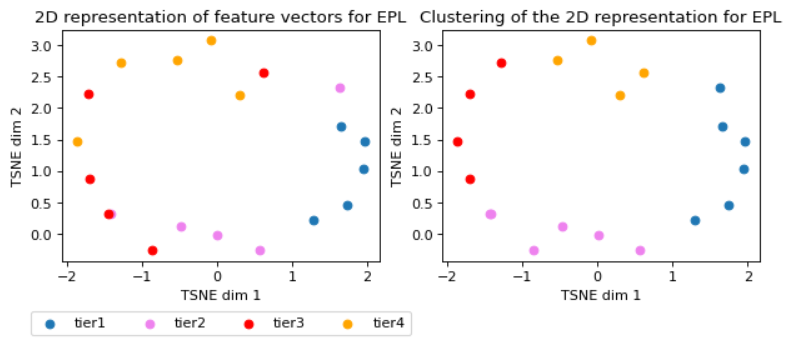
\includegraphics[width=1\textwidth]{figures/2d_epl.png}
    \caption{2D representation of away feature vectors with TSNE for EPL. The teams are divided into tiers according to the final results of the predicted season on the left and clustered by k-means on the right.}
    \label{fig:epl_2d}
\end{figure}

The same can be seen in Figures~\ref{fig:bl_2d},~\ref{fig:llpd_2d},~\ref{fig:sa_2d},~\ref{fig:bsa_2d} for BL, LLPD, SA, and BSA, respectively. In SA, the teams from the same tiers are close together, and the division by tiers looks very similar to the clustering. In BL and LLPD, at least teams of some tiers are close together, but in BSA, only tier 1 and tier 4 teams are on the same half, and teams from other tiers are mixed up.

\begin{figure}[h]
    \centering
    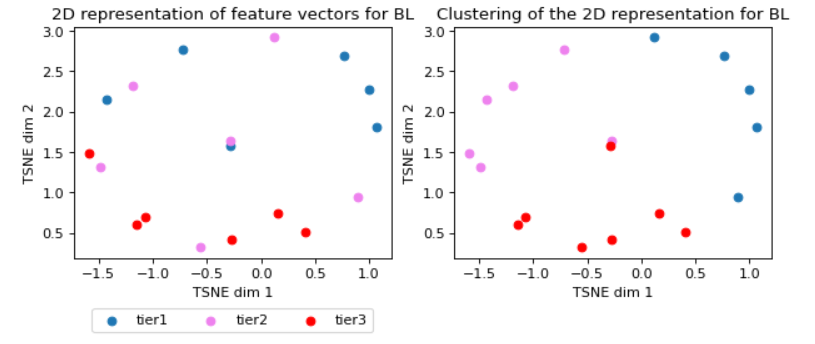
\includegraphics[width=1\textwidth]{figures/2d_bl.png}
    \caption{2D representation of away feature vectors with TSNE for BL.}
    \label{fig:bl_2d}
\end{figure}

\begin{figure}[h]
    \centering
    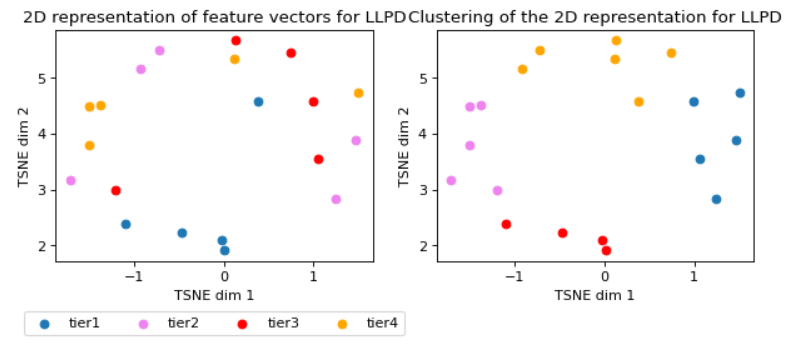
\includegraphics[width=1\textwidth]{figures/2d_llpd.png}
    \caption{2D representation of away feature vectors with TSNE for LLPD.}
    \label{fig:llpd_2d}
\end{figure}

\begin{figure}[h]
    \centering
    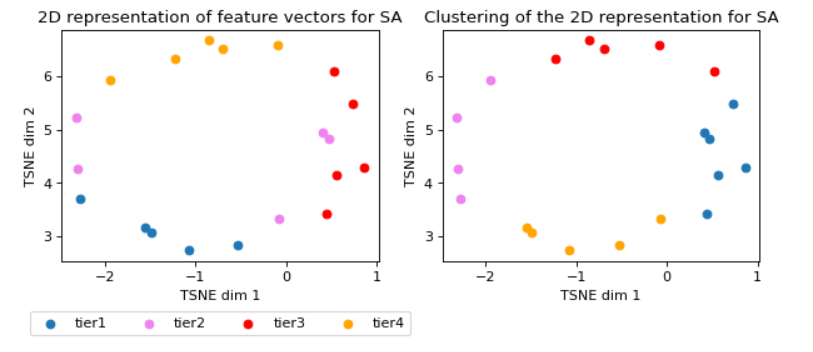
\includegraphics[width=1\textwidth]{figures/2d_sa.png}
    \caption{2D representation of away feature vectors with TSNE for SA.}
    \label{fig:sa_2d}
\end{figure}

\begin{figure}[h]
    \centering
    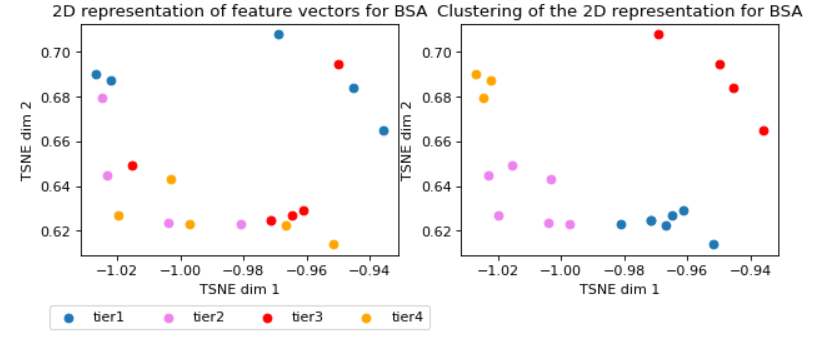
\includegraphics[width=1\textwidth]{figures/2d_bsa.png}
    \caption{2D representation of away feature vectors with TSNE for BSA.}
    \label{fig:bsa_2d}
\end{figure}


\begin{conclusion}
In my master's thesis, I predicted the outcomes of football matches from different leagues using various machine learning techniques. I applied tensor completion to this task, which had not been done before. I created a tensor completion model that used only match results from previous seasons for the prediction. This innovative approach, which treats the outcomes of all seasons as a 3D tensor, brings a brand new perspective to the subject.

Firstly, I conducted extensive research on the literature related to predicting football results and sports results in general using machine learning. From the researched papers, I chose a few of them as baselines. I described the chosen works and pointed out the similarities and differences between them and my thesis. I also researched several tensor completion algorithms, from which I then chose the best one for the prediction.

From the literature review, I selected Linear Regression, a model consisting of PCA and NB, ANN, and matrix factorization as baselines. I studied and described these methods in detail and gained a deep understanding of the models.

Moreover, I collected data from seasons 1993/94 to 2018/19 of EPL, BL, LLPD, SA, and BSA. I obtained the data from various sources and created different feature sets for different models. Moreover, I analyzed the dataset and found that the overall percentage of home wins is around 47\%, and away wins and draws both form about 26-27\%.

Additionally, I implemented an algorithm that uses tensor completion for the prediction. This algorithm does not take into account any statistics from games, only the outcomes. I also implemented the baselines according to relevant papers, with features, architecture, and the amount of data as similar as possible to the originals. To better compare the tensor completion model with the baselines, I created a Win-loss feature set, which only contains features gathered from the results. The accuracy of the model utilizing tensor completion was comparable or higher than the accuracy of the baselines.

Lastly, I extracted feature vectors from the last season using the tensor completion algorithm and SVD. These tensor completion embeddings were then added to the feature sets to improve the performance of other models. The accuracy of the ANN improved, but the accuracy of the other methods did not, probably due to the nonlinear dependencies in the vectors, which only the ANN can handle. I also plotted these vectors into 2D using TSNE. Especially for SA, the positions of the plotted vectors resemble the standings of the teams in the final table.

Future directions for this thesis would be to apply the tensor completion model and embeddings to other football leagues, as well as to other sports such as ice hockey, basketball, or American football. Moreover, it would be beneficial to apply the inductive tensor completion method to implement additional information into the model. Additionally, implementing other methods for football prediction and adding the feature vectors to their inputs to improve their accuracy would be another future direction.
\end{conclusion}

\bibliographystyle{iso690.bst}
\bibliography{ref}

\appendix



\chapter{Contents of CD}\label{app:CDcontent}

\begin{figure}
	\dirtree{%
		.1 readme.txt\DTcomment{the file with CD contents description}.
		.1 data\DTcomment{the data files directory}.
            .2 results\_files\DTcomment{the files with results and statistics of the matches}.
            .2 feature\_matrices\DTcomment{the home and away feature matrices}.
		.1 src\DTcomment{the directory of source codes}.
		.2 analysis\DTcomment{the analysis of dataset and feature vectors}.
		.2 implementation\DTcomment{the implementations of the models}.
            .2 functions\DTcomment{the files with different functions}.
            .2 pyten.rar\DTcomment{the compressed file of the Pyten package}.
		.2 thesis\DTcomment{the directory of \LaTeX{} source codes of the thesis}.
		.3 figures\DTcomment{the thesis figures directory}.
		.3 *.tex\DTcomment{the \LaTeX{} source code files of the thesis}.
		.1 text\DTcomment{the thesis text directory}.
		.2 thesis.pdf\DTcomment{the Diploma thesis in PDF format}.
		.2 thesis.ps\DTcomment{the Diploma thesis in PS format}.
	}
\end{figure}


\end{document}

